% Capítulo 2
\chapter{Estado da Arte}
\label{Capitulo2}

\begin{flushright}
\textit{```You are entering a world of pain.''} \\[0.5em]
--- Walter Sobchak, \textit{The Big Lebowski}
\end{flushright}
Tendo em conta a experiência do autor como professor numa escola secundária, neste capítulo procura-se fazer o enquadramento das principais dificuldades que a Educação (digital) atravessa em Portugal e discutir em que medida a integração da tecnologia digital na educação é essencial para criar ambientes de aprendizagem mais eficazes e adaptados à evolução do panorama digital. Explora-se o potencial de tecnologias, como os laboratórios remotos, para o desenvolvimento de experiências de aprendizagem personalizadas e reflete-se sobre a forma como podem ajudar a suprir estas mesmas dificuldades.
Face a isto, discute-se a ascensão do \textit{eLearning}, particularmente no contexto da abordagem \acrshort{stem}, assim como a evolução da educação das salas de aula tradicionais para ambientes virtuais, enfatizando as oportunidades e possibilidades de aprendizagem alargadas oferecidas pelo \textit{eLearning}

\section{Transformação digital na educação}
\label{sec:transformaçãodigital}
A educação está a sofrer grandes mudanças a nível tecnológico, social e humano. Estas foram impulsionadas pela \acrfull{covid-19}, que expôs as fragilidades em termos de gestão e capacitação dos recursos tecnológicos e do eLearning\footnote{Jay Cross, é conhecido por ter ``cunhado'' pela primeira vez o termo \textit{eLearning}\cite{jaycross}. Por isso, nesta dissertação, o termo será sempre referido desta forma, em vez de \textit{e-Learning}}. O sistema educativo português apresenta ainda várias fragilidades que ficaram particularmente evidentes nesse contexto. Ainda assim, graças a um grande esforço coletivo, conseguiu responder de forma imediata a este enorme obstáculo. Num curto espaço de tempo, o ensino presencial e o contacto humano foram substituídos pelo ensino à distância. Estávamos pronto para isto?

Antes da pandemia, no Ensino Básico, as tecnologias digitais eram mais frequentemente utilizadas como meio de comunicação do que como ferramenta pedagógica~\cite{oecd_using_2021}. Nas últimas duas décadas aproximadamente, Portugal já introduziu programas para abordar a digitalização na educação. O programa de digitalização contemplado no Plano de Ação para a Transição Digital (Resolução do Conselho de Ministros n.º 30/2020, de 21 de abril) prevê, entre outras medidas, uma forte aposta na formação digital dos professores, no desenvolvimento digital das escolas e na disponibilização de recursos educativos digitais \cite{transicaodigital, capacitacaodigital}.

No mundo de hoje, cada vez mais digital, apesar de em 2024 o número de utilizadores da Internet se situar nos 5,5 mil milhões, ainda existem 2,6 mil milhões de pessoas sem acesso à Internet, como se pode observar no gráfico retirado do relatório ``\textit{ITU Facts \& Figures 2024}'' e apresentado na Figura~\ref{fig:numutilizadoresnet} \cite{broadbandcomission, itu2024facts}.

\begin{figure}[hbtp]
    \centering
    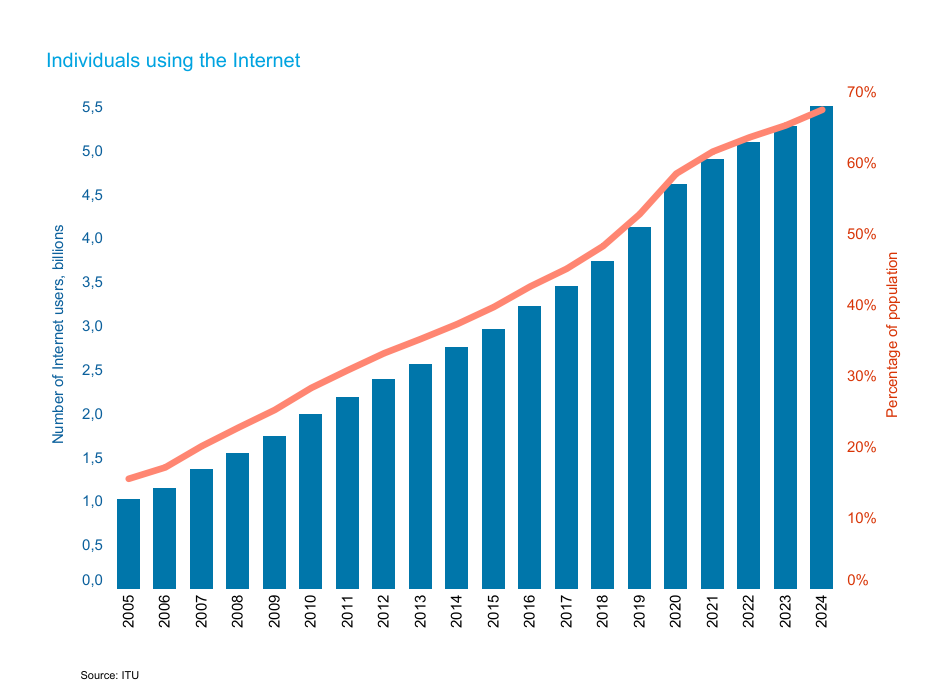
\includegraphics[width=0.65\textwidth]{figures/ITU-InternetUse.png}
    \caption{Número de utilizadores da Internet em todo o mundo, 2024 \cite{itu2024facts}}
    \label{fig:numutilizadoresnet}
\end{figure}
Este problema reduz o acesso a um mundo de informações disponíveis \textit{online} e limita o potencial de aprendizagem e crescimento, para não falar das competências digitais de que as pessoas necessitam para aprender e melhorar as suas vidas.
A crise da \acrshort{covid-19} mostrou-nos como a ligação à Internet é crucial para as actividades quotidianas, como o trabalho e a aprendizagem. Hoje, mais do que nunca, é necessário reforçar as infra-estruturas nacionais para garantir que a conetividade esteja mais amplamente disponível. Igualmente importante é reforçar os planos de conetividade das escolas e investir numa aprendizagem de qualidade, a fim de melhorar o acesso à educação, os resultados da aprendizagem e o potencial de ganhos dos jovens, bem como o desenvolvimento socioeconómico das suas comunidades e países~\cite{TheDigitransf}.

Ainda que não constitua objetivo central desta dissertação proceder a uma análise exaustiva ao ``Digital Decade 2024 Country Report'' \cite{DESI2024}, a consulta de alguns indicadores-chave permite constatar que, em 2023, Portugal registou uma taxa de 55,97\% da população com, pelo menos, competências digitais básicas — ligeiramente acima da média da União Europeia (55,56\%). Este progresso tem sido acompanhado por um crescimento sustentado no número de especialistas em \acrshort{tic}.
Contudo, o desempenho global de Portugal na dimensão Capital Humano, segundo o índice \acrshort{desi}, continua a posicionar-se abaixo da média europeia, como evidenciado no gráfico geral apresentado na Figura~\ref{fig:all_individuals}. A distribuição etária representada na Figura~\ref{fig:individuals} demonstra que Portugal se encontra entre os países com menor desempenho nas faixas etárias mais elevadas, revelando que persistem desafios significativos noutros indicadores que continuam a comprometer esta dimensão estratégica para a transição digital.

\begin{figure}[hbtp]
	\centering%
		\centering
		\subfloat[\centering Todos os individuos\label{fig:all_individuals}]{{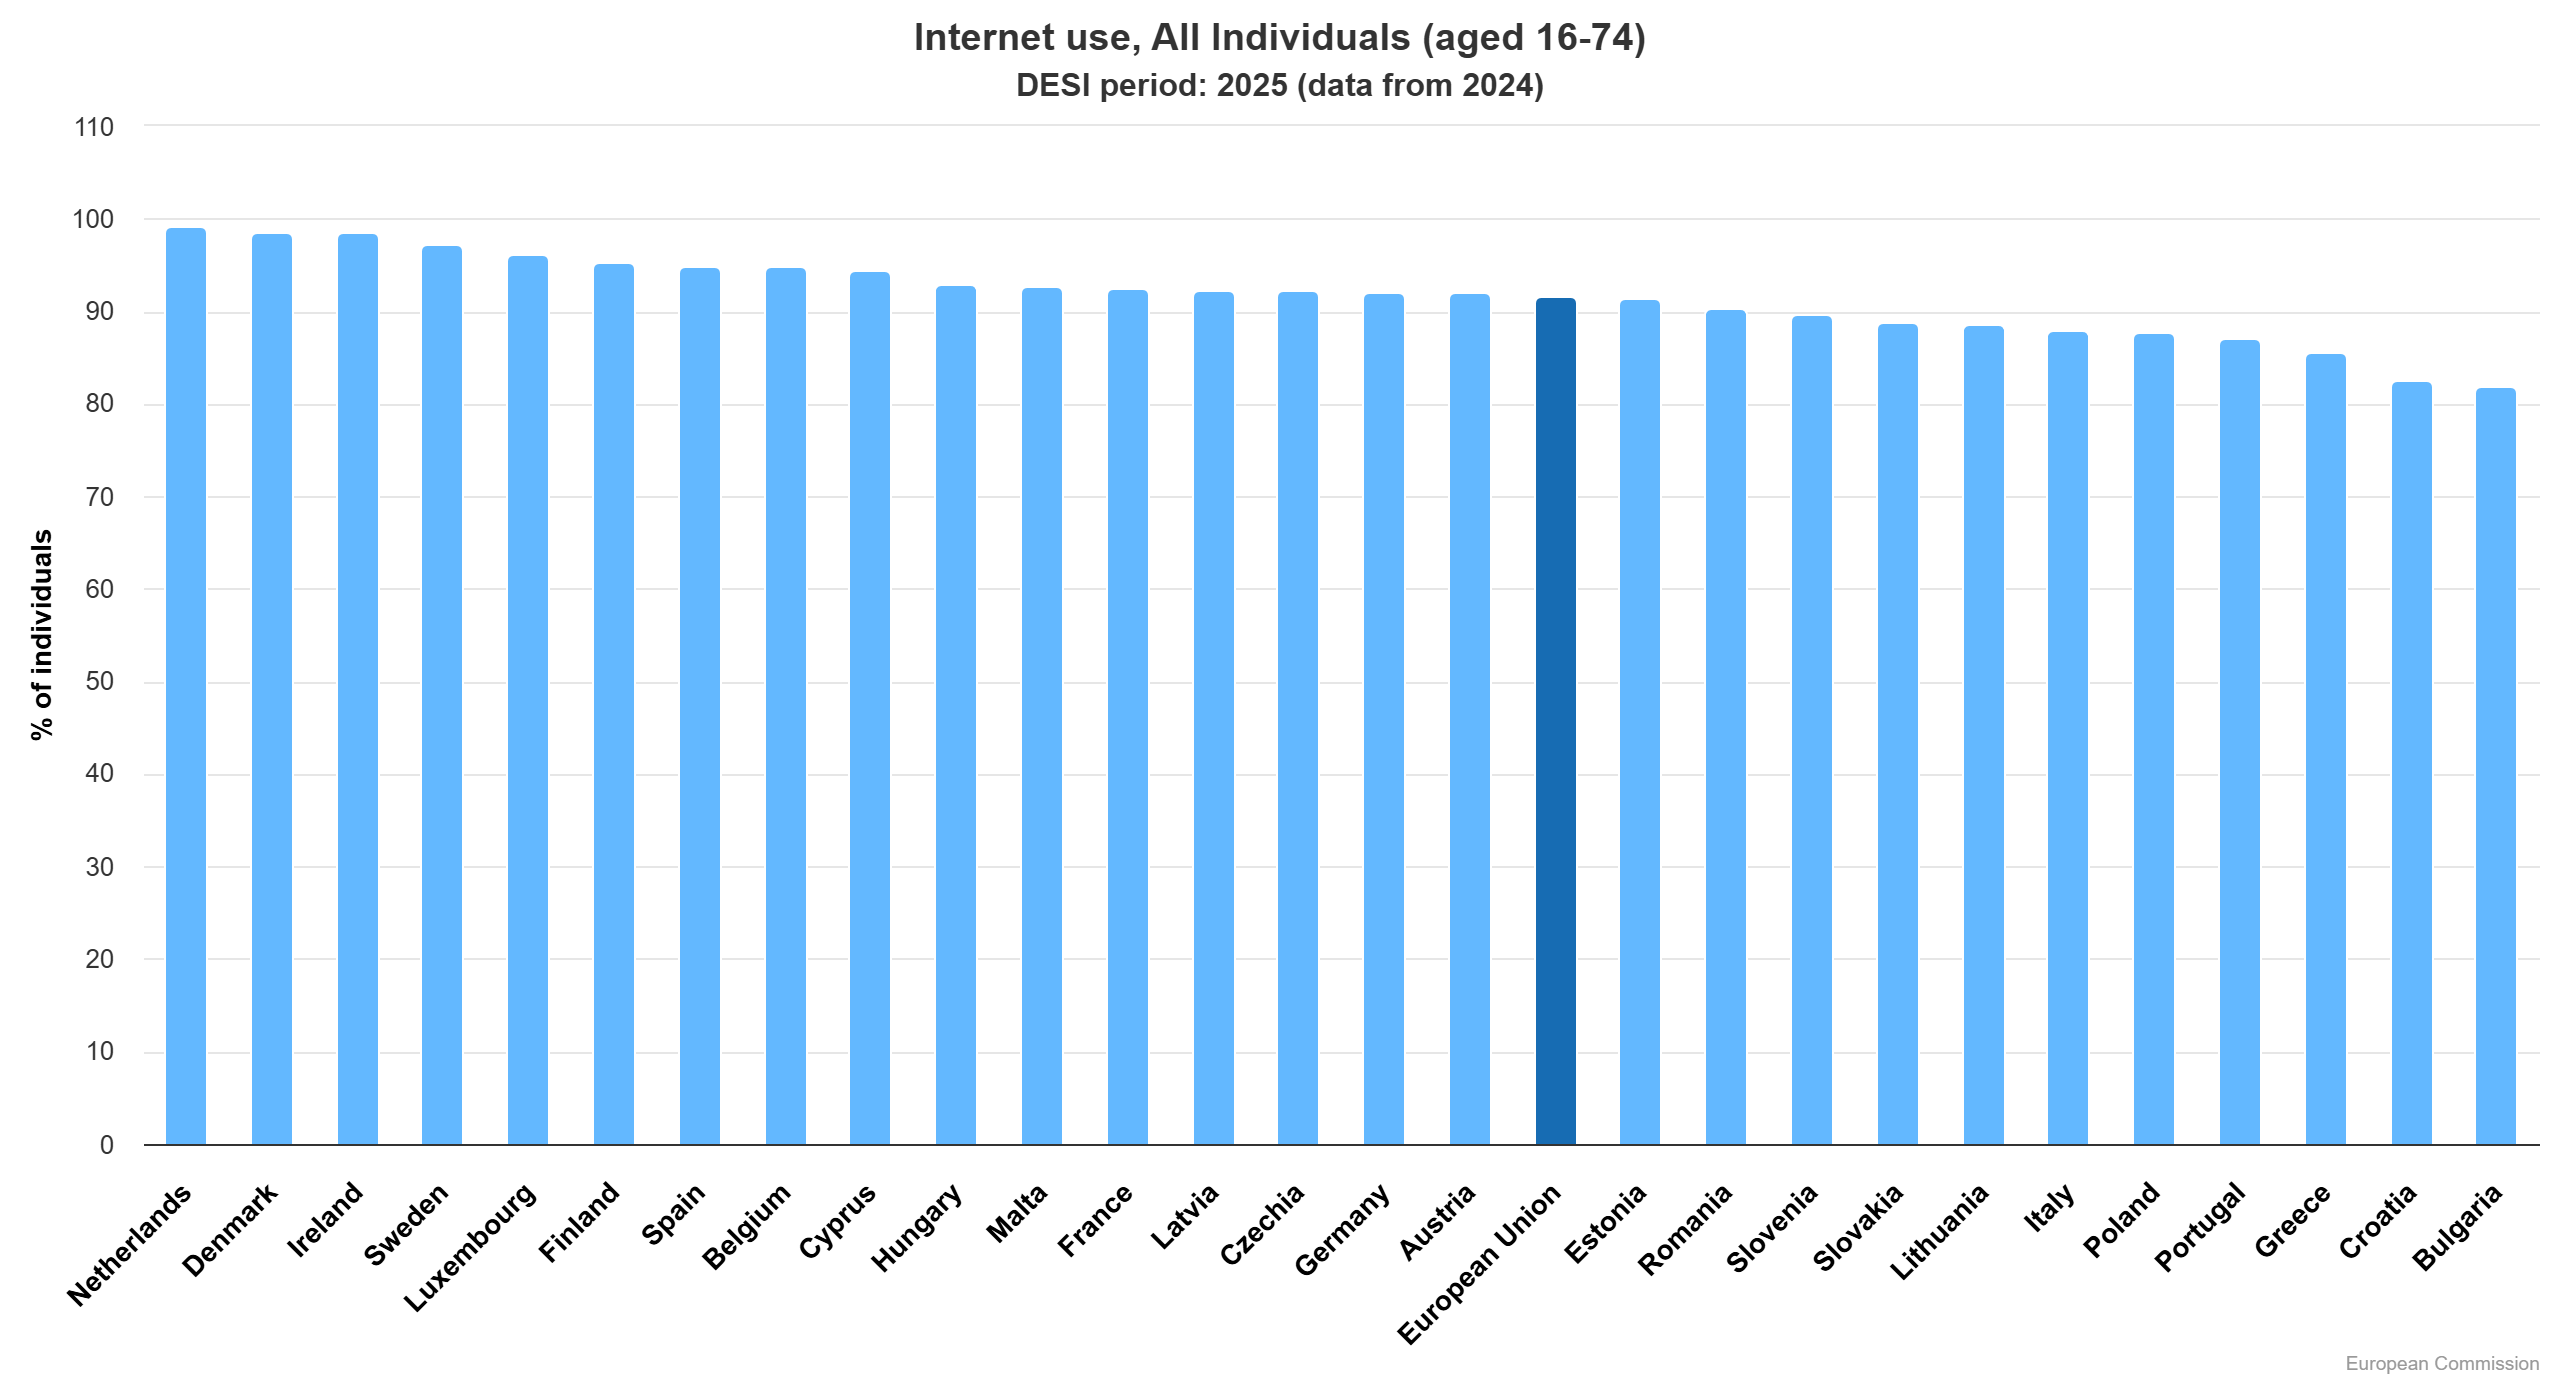
\includegraphics[width=6.3cm]{figures/internet-use-all-individ.png} }}%
		\qquad
		\subfloat[\centering Individuos entre 55 e 74 anos de idade\label{fig:individuals}]{{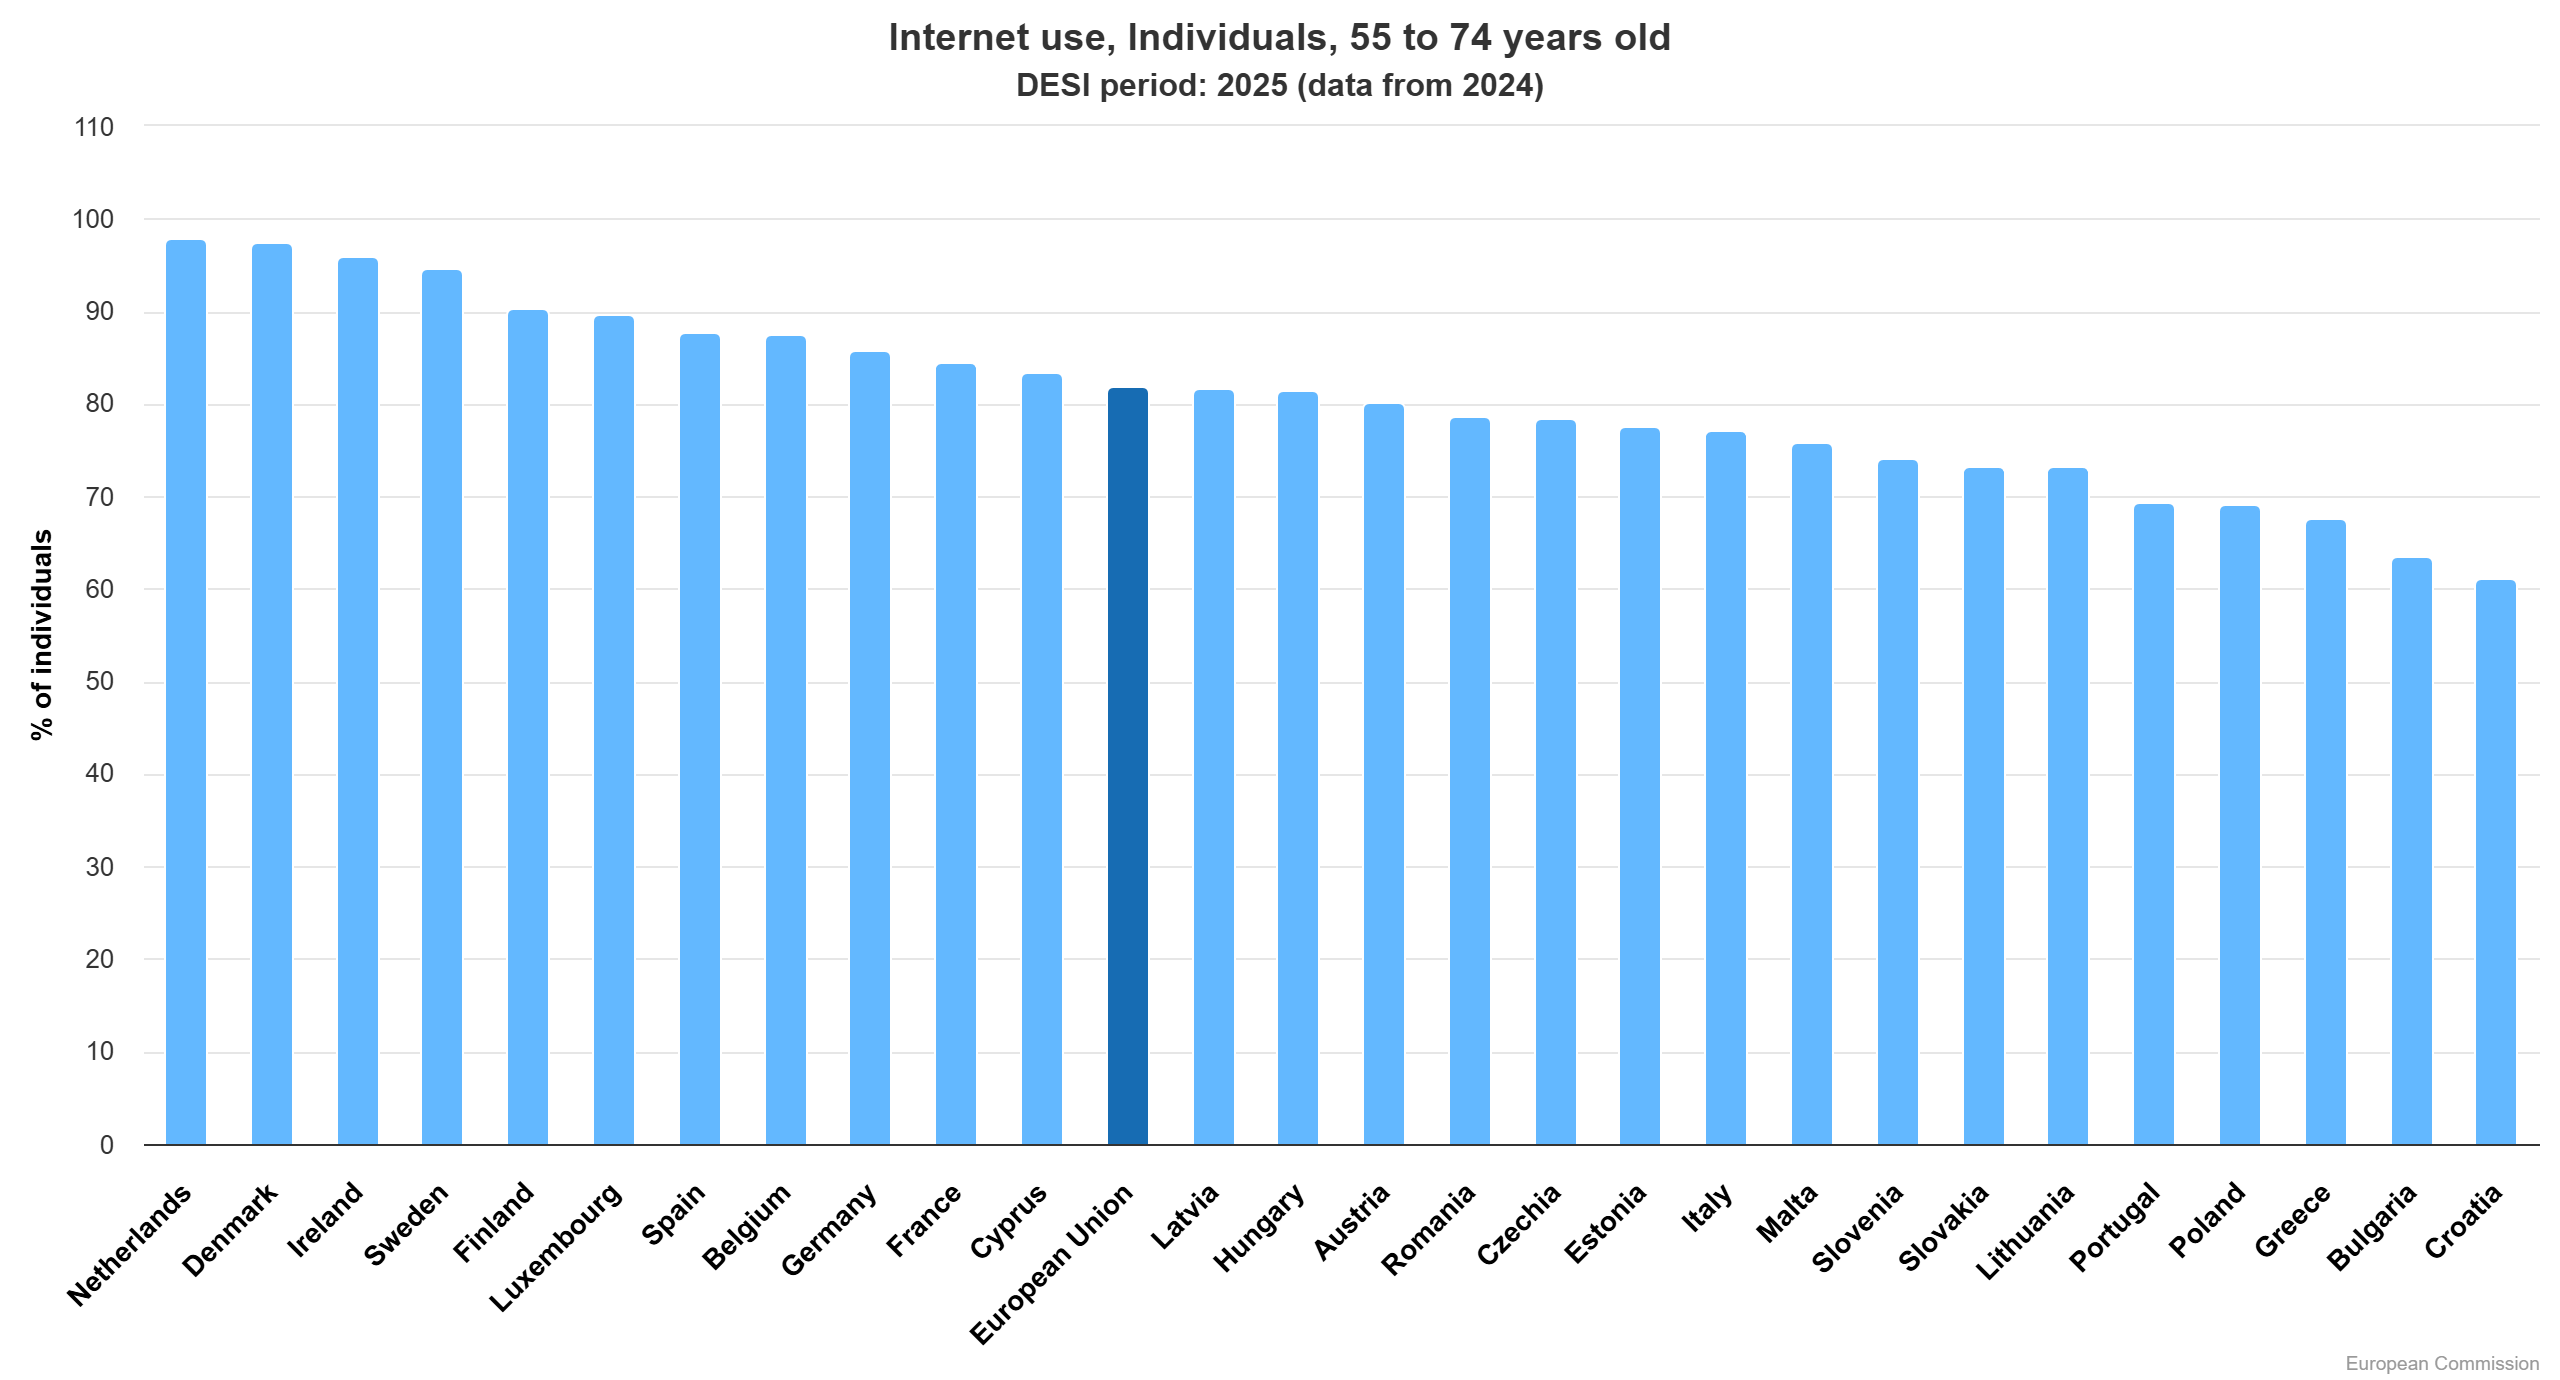
\includegraphics[width=6.3cm]{figures/internet-use-individuals-54-74.png} }}%
		\caption{Dimensão Capital Humano, 2024 \cite{itu2024facts}}%
		\label{fig:capitalhumano}%
	\end{figure}

O mesmo relatório enfatiza que, apesar do avanço nas competências básicas, são necessários esforços redobrados para que Portugal atinja a meta europeia de 80\% da população com competências digitais básicas até 2030 e supere os seus défices na dimensão global do Capital Humano \cite{DESI2024}.

Pode, assim, concluir-se que esta falta de competências básicas foi agravada pela pandemia. De acordo com o relatório ``\textit{Youth \& COVID-19: Impacts on jobs, education, rights and mental well-being}'' \cite{impactocovideducacao}, 65\% dos jovens afirmaram ter aprendido menos desde o início da pandemia, devido à transição das aulas presenciais para o regime \textit{online} durante o confinamento. Apesar dos esforços para manter os estudos, metade considerou que ficou para trás, e 9\% temeu reprovar devido às dificuldades sentidas. A situação foi ainda mais grave entre os jovens de países com baixos rendimentos, devido ao acesso limitado à Internet, à falta crítica de equipamentos e, em alguns casos, à ausência de um espaço adequado para aprendizagem em casa \cite{impactocovideducacao}.

Com base nestes resultados, o estudo conclui que ``os desafios colocados pela transição para o ensino fora da sala de aula e em casa'' foram enormes. Mesmo quando as instituições conseguiram fazer a transição para a aprendizagem \textit{online}, os professores, formadores e estudantes podem não ter tido a capacidade de ``garantir a continuidade da aprendizagem''. Entre os factores que dificultam a eficácia do ensino \textit{online} contam, como já foi referido: baixos níveis de acesso à Internet; lacunas nas competências digitais; incapacidade de ensinar e aprender à distância; falta de equipamento informático em casa; falta de espaço; falta de materiais preparados para o \textit{eLearning}; e falta de trabalho de grupo e de contacto social - ambos componentes fundamentais do processo de aprendizagem.

Enquanto docente do ensino secundário e diretor de turma, com responsabilidades tanto junto do corpo docente como dos alunos, foi possível observar diversas dificuldades enfrentadas pelos estudantes, nomeadamente a ausência de um computador pessoal, a falta de acesso à Internet ou a existência de uma ligação extremamente lenta. Registaram-se, inclusivamente, casos de alunos que participaram nas aulas através do telemóvel. Do lado dos docentes, verificou-se um desafio considerável, sobretudo devido à falta de experiência prévia no ensino à distância e às dificuldades em identificar e utilizar adequadamente as diversas ferramentas \textit{online}. A correspondente curva de aprendizagem revelou-se lenta e exigente para muitos deles.

Esta realidade não se verificou apenas em Portugal, mas estendeu-se a nível global. Em meados de março de 2020, escolas e instituições de ensino em todo o mundo foram encerradas, e os alunos de todos os níveis passaram a assistir às aulas e a interagir com os professores através de videoconferências e outras ferramentas digitais. A \acrfull{unesco} apoiou a implementação de programas de ensino à distância em larga escala, recomendando aplicações e plataformas educativas gratuitas que pudessem ser utilizadas por escolas e professores para assegurar a continuidade pedagógica. A organização partilhou ainda boas práticas para o uso de tecnologias móveis de baixo custo com fins educativos, com o objetivo de atenuar os impactos negativos da interrupção do ensino presencial \cite{unesco}.

Do ponto de vista da prática pedagógica em contexto de sala de aula, especialmente nas disciplinas laboratoriais — como é o caso da eletrónica —, as aulas à distância mostraram-se particularmente desadequadas. Um exemplo evidente foi a substituição do contacto direto com materiais físicos, como a placa de ensaio (também conhecida por breadboard) e os componentes eletrónicos reais, pelo uso de simuladores \textit{online}, como o \href{https://www.multisim.com/}{Multisim} e o \href{https://www.falstad.com/circuit/}{Falstad}. Embora estes simuladores já fossem utilizados como complemento às actividades presenciais, o seu uso exclusivo limitou fortemente a experiência prática dos alunos, que deixaram de poder manipular fisicamente os circuitos - um aspecto central para a consolidação de competências técnicas nesta área. Em Agosto de 2020, numa citação incluída num artigo publicado no \textit{Diário de Notícias}, um aluno afirmava:
\begin{center}
    ``\textit{As aulas de laboratório foram as que menos sentido fizeram para mim, pois fazer relatórios e cálculos sobre experiências que não fizemos, sem adquirir/desenvolver as competências e técnicas que é suposto esta componente da disciplina nos dar, é um pouco ridículo}'' \cite{impactonegativocovid}.
\end{center}

Assim, a resposta à questão colocada anteriormente é: não, ninguém estava preparado para estas mudanças nem para o ensino \textit{online} e o \textit{eLearning}.

Nos últimos anos, Portugal tem investido significativamente, não só na educação digital mas também em diversas iniciativas, reconhecendo a importância das competências digitais para o futuro dos seus cidadãos e para a competitividade do país. No contexto nacional, o \acrfull{prr} previu a entrega de computadores portáteis a todos os alunos e docentes do ensino básico e secundário. Estava inicialmente prevista a distribuição de 600 mil computadores com acesso à Internet; contudo, a implementação ficou aquém das expectativas. Em 2023, a \acrfull{cnaprr} classificava como ``preocupante'' a evolução da iniciativa Escola Digital \cite{PRREntregacomputadores}. Até essa data, apenas cerca de 70\% dos equipamentos tinham sido efetivamente entregues. A principal razão prendeu-se com a exigência de um compromisso por parte dos encarregados de educação, que teriam de reembolsar o valor dos equipamentos caso não os devolvessem nas mesmas condições, dificultando a aceitação do programa. Acrescem ainda dificuldades logísticas identificadas por diversas escolas \cite{PRREntregacomputadores}. A estas limitações somam-se decisões políticas recentes que não parecem alinhar-se com os objetivos da transição digital. No início do ano letivo de 2024/2025, foi reportado que milhares de alunos e docentes ficaram sem acesso aos hotspots de Internet integrados nos kits digitais escolares, medida justificada pela tutela como sendo transitória, mas que afetou diretamente a continuidade digital no processo de ensino-aprendizagem. Esta alteração comprometeu não só a equidade no acesso, como também a eficácia dos recursos já distribuídos, dificultando o cumprimento dos objetivos traçados no Plano de Acção para a Transição Digital~\cite{ExecutiveDigest2024}.

Lançado em 2017, o Plano Nacional de Competências Digitais (INCoDe.2030)~\cite{incode2030} constitui uma iniciativa estratégica do governo português com o objetivo de reforçar a literacia digital da população em geral. Estruturado em cinco eixos fundamentais — inclusão, educação, qualificação, especialização e investigação — o plano orienta um conjunto alargado de políticas públicas e iniciativas destinadas à promoção das competências digitais ao longo da vida. No âmbito deste plano foi criado o Observatório das Competências Digitais, uma plataforma de monitorização e análise que sistematiza e disponibiliza informação sobre as diversas ações e programas desenvolvidos no contexto do INCoDe.2030. Entre as iniciativas registadas pelo Observatório destacam-se projetos como “Eu Sou Digital”, \textit{Apps for Good} e a iniciativa Ensico \cite{observatorio2030}, representando exemplos concretos da operacionalização das metas estabelecidas pelo plano.

Em junho de 2025, a \acrshort{cnaprr} apresentou o quinto relatório relativo à execução do \acrshort{prr}. Este documento destaca os investimentos estratégicos associados à transição digital, bem como os resultados esperados, entre os quais se salientam a ``a diminuição das desigualdades no acesso à tecnologia'' e ``melhorias na eficiência e qualidade dos processos de ensino''. Entre os investimentos identificados no relatório, orientados para a modernização das infraestruturas escolares, incluem-se: a aquisição de videoprojectores, a implementação dos \acrfull{led}, a ampliação das redes de área local sem fios, o reforço da conectividade à Internet através da rede alargada da Educação, bem como o Projeto Redimensionar a ligação das escolas a essa rede, com vista à melhoria da largura de banda e da fiabilidade do acesso \cite{cnaprr2025}.

Complementarmente, no estudo de caso desenvolvido por Wastiau et al. (2024)~\cite{estrategiatransdigital}, são analisadas outras iniciativas que sustentam a transição digital no sector educativo, com destaque para o Programa Nacional de Promoção do Sucesso Escolar (PNPSE), a Estratégia Nacional de Educação para a Cidadania (ENEC), consagrada no Decreto-Lei n.\textsuperscript{o}~55/2018, e o Regime Jurídico da Educação Inclusiva, estabelecido pelo Decreto-Lei n.\textsuperscript{o}~54/2018. Segundo os autores, estas políticas ``(...) orientam e são, por sua vez, fortalecidas pela estratégia de transição digital adoptada em 2020''~\cite{estrategiatransdigital}.

Os desafios para alunos e professores foram enormes, a adaptação ao processo de ensino/aprendizagem \textit{online} teve de ser feita muito rapidamente e os recursos digitais tornaram-se a ``tábua de salvação'' da educação. No entanto, as oportunidades que as tecnologias digitais oferecem vão muito além do apoio de emergência utilizado durante a pandemia. Actualmente, está disponível um número infinito de possibilidades, novas respostas para o quê, como e quando as pessoas aprendem \cite{oecd_state_2021}.

A forma de pensar dos estudantes de hoje é também muito diferente da de há trinta anos. De uma forma mais particular, o pensamento mudou muito desde que a Internet e os recursos digitais começaram a tornar-se massivos. É essencial que os alunos possam aceder à tecnologia e utilizá-la para se desenvolverem ainda mais e a lição mais importante de todas é: permitir-lhes compreender o que fazer com a informação e os recursos que estão à sua disposição de tantas formas diferentes. Esta nova adaptação educativa (ou deveria chamar-se ``evolução''?) ``também adapta a aprendizagem aos estilos de aprendizagem pessoais com uma granularidade e precisão muito maiores do que qualquer ambiente de sala de aula tradicional pode fazer. Do mesmo modo, laboratórios virtuais dão aos alunos a oportunidade de conceber, realizar e aprender com as experiências, em vez de se limitarem a aprender sobre elas'' \cite{oecd_state_2021}.

Por outro lado, os professores devem desenvolver a sua literacia digital, para melhor dominarem estas novas ferramentas na sala de aula, de forma a ajudarem os alunos a construírem o seu próprio conhecimento. Assim, é evidente que a Educação, como um todo, precisa de se inserir neste contexto que está cada vez mais presente no quotidiano de todos. O mundo é cada vez mais dominado pela tecnologia (\ldots e, nos tempos actuais, o domínio da Inteligência Artificial já se faz sentir). Milhares de milhões de dispositivos físicos em todo o mundo estão agora ligados à Internet, todos recolhendo e partilhando dados. Actualmente, os circuitos integrados — ou microprocessadores e \acrfull{microcontroladores}, consoante a aplicação — são produzidos a baixo custo, e a ubiquidade das redes sem fios permite ligar praticamente qualquer objecto, desde algo tão pequeno como um comprimido até algo tão grande como um avião. A esta rede global de dispositivos interligados, com capacidade de recolher e trocar dados em tempo real, dá-se o nome de Internet das Coisas (\acrfull{iot}) \cite{IoT}.

Por conseguinte, a informação e os recursos estão “na ponta dos dedos de todos” e à distância de um clique.

\begin{center}
    ``\textit{Chegou o momento de os países aproveitarem as lições da pandemia para reconfigurarem as pessoas, os espaços, o tempo e a tecnologia, de modo a criarem ambientes educativos mais eficazes e eficientes}'' \cite{thestateofeducation}.
\end{center}

Se reflectirmos sobre esta ideia em contexto educativo e acrescentarmos o facto de o ensino da electrónica em Portugal passar pelo ensino profissional e se o objetivo é a evolução e inovação no processo de ensino/aprendizagem, é necessário proporcionar a todos os intervenientes as condições e ferramentas necessárias para que o trabalho possa ser desenvolvido e, consequentemente, os alunos realmente aprendam. Praticamente todas as aprendizagens e futuros empregos exigirão um certo nível de competências e aptidões digitais. A constante evolução tecnológica exige o desenvolvimento de competências ao longo da vida \cite{Digitale13:online}.

O esforço na evolução da educação digital em Portugal, e consequente aumento do indíce \acrshort{desi} de Capital Humano,  pode ser aferida pelas crescentes iniciativas governamentais e adopção de tecnologias digitais nas escolas e universidades. Este esforço é materializado através de várias iniciativas e programas governamentais que visam aumentar a literacia digital, integrar a tecnologia no sistema educacional, capacitar professores e preparar os estudantes para a era digital. ``As medidas de apoio aos objetivos digitais representam um montante que corresponde a 22\% da dotação total do plano, ultrapassando o limiar de 20\% definido pela regulamentação europeia'' \cite{Transicaodigitalprr}.
\begin{comment}
SE CALHAR TERMINAVA AQUI

No entanto, no meio destas oportunidades criadas, ainda há alguns desafios que precisam de ser ultrapassados. A desigualdade no acesso à tecnologia ainda é uma barreira significativa \cite{desigualdades}, especialmente em áreas rurais e entre famílias de baixos rendimentos. A formação contínua dos professores também necessita de maior suporte, assim como a atualização constante dos recursos digitais disponíveis \cite{afirmacaodigital, problemasprovas}. 
\end{comment}

\section{eLearning e abordagem STEM} %The main chapter title
%\chaptermark{O \textit{Template}}	%Short version for page header. Comment if not needed
\label{sec:elearningstem}	%For referencing the chapter elsewhere, use \ref{Chapter2} 

%%%%%%%%%%%%%%%%%%%%%%%%%%%%%%%%%%%%
Após a análise dos investimentos em infraestruturas digitais e das políticas educativas associadas à transição digital, importa agora aprofundar duas abordagens fundamentais neste contexto: o \textit{eLearning} e a abordagem STEM (Ciência, Tecnologia, Engenharia e Matemática). Estas abordagens, embora distintas nas suas origens, revelam-se hoje profundamente interligadas, sobretudo quando integradas em ambientes de aprendizagem mediados por tecnologia.

A evolução recente da educação digital foi particularmente acelerada com a pandemia da \acrshort{covid-19}, que impulsionou a adopção de recursos digitais a uma escala sem precedentes. O \textit{eLearning}, até então complementar ao ensino presencial, tornou-se não apenas comum, mas necessário. Assistiu-se, assim, a uma migração generalizada do modelo tradicional de sala de aula para ambientes virtuais de aprendizagem, baseados em plataformas digitais. Esta transformação não apenas democratizou o acesso à educação, como também ampliou as possibilidades pedagógicas, abrangendo formatos como cursos \textit{online}, laboratórios virtuais e remotos e simuladores digitais. Neste contexto, torna-se pertinente reflectir sobre como o \textit{eLearning} se articula com abordagens como a \acrshort{stem}, especialmente no que se refere ao desenvolvimento de competências digitais, científicas e tecnológicas. A integração de laboratórios remotos, simuladores e ambientes experimentais digitais surge, assim, como um eixo estruturante para uma educação inovadora, inclusiva e tecnicamente 
atualizada.

\subsection{Uma questão de conceitos}
O conceito de \textit{eLearning} tem sido amplamente discutido, sendo objeto de múltiplas definições ao longo das últimas décadas. Esta diversidade não é apenas semântica, mas reflete também os diferentes contextos de aplicação e as abordagens teóricas subjacentes. Em 2004, Jay Cross no seu artigo ``\textit{An Informal History of eLearning}''~\cite{jaycross}, discute a natureza fluida e a evolução deste modelo. Cross apresenta o \textit{eLearning} como uma visão para a transformação da formação empresarial, destacando o seu carácter informal e descentralizado.  No entanto, num estudo intitulado ``O e-Learning no Ensino Superior: um caso de estudo'' \cite{eLearningenssup}, Magano et al. (2008), generalizam a definição dada por Maria João Gomes no seu artigo sobre reflexões em torno do \textit{eLearning} \cite{gomes_e-learning_2005}, considerando que este ``(\ldots) corresponderá a qualquer metodologia de ensino/aprendizagem que integre actividades, suportadas por \acrshort{tic}, essenciais para atingir os objectivos de aprendizagem definidos.''. No mesmo artigo, Maria João Gomes defende que ``(\ldots) o termo e-learning deve ser adoptado como menos centrado nos aspectos tecnológicos e mais próximo das potencialidades pedagógicas decorrentes da utilização das ``tecnologias de rede'' na concepção de situações baseadas na interacção e colaboração, no sentido da construção de aprendizagens significativas''.

Assim, é evidente que não existe um consenso unívoco sobre o significado de \textit{eLearning}. Esta multiplicidade de definições resulta das diversas perspetivas, interesses e concepções dos diferentes intervenientes — académicos, técnicos, políticos e pedagógicos — que, de diferentes formas, têm contribuído para o desenvolvimento deste domínio.

Para ilustrar ainda mais essa diversidade de entendimentos, destaca-se a definição apresentada no ``Convite à apresentação de propostas DG EAC/46/02'' \cite{comissao197_07}, que descreve o \textit{eLearning} como ``(...) a utilização das novas tecnologias multimédia e da Internet para melhorar a qualidade da aprendizagem, facilitando o acesso a recursos e serviços, bem como o intercâmbio/interação e a colaboração à distância.'' Esta visão aproxima-se de uma concepção de aprendizagem assente na comunicação e na colaboração \textit{online}, como referida também por Maria João Gomes \cite{gomes_e-learning_2005}.

Uma das principais vantagens do \textit{eLearning} é a flexibilidade que oferece. Os estudantes podem aprender ao seu próprio ritmo e horário, o que é particularmente útil para aqueles que têm outras responsabilidades, como o trabalho ou a assistência à família. Além disso, o \textit{eLearning} também pode ocorrer a partir de qualquer lugar, desde que haja uma ligação à Internet, o que permite aos alunos estudar a partir de casa ou de qualquer outro lugar que lhes seja conveniente.

Outra vantagem do \textit{eLearning} é que permite o acesso a uma grande variedade de recursos e materiais de aprendizagem, incluindo vídeos, textos, actividades interactivas, fóruns de discussão, laboratórios virtuais e remotos, entre outros. Estes recursos podem ser actualizados e adaptados rapidamente de acordo com as necessidades dos alunos e professores, garantindo que os conteúdos estão sempre actualizados e são relevantes.

O \textit{eLearning} também pode ser uma forma eficaz de personalizar a aprendizagem, permitindo que os alunos se concentrem nas áreas em que precisam de mais ajuda e avancem rapidamente nas áreas em que já têm conhecimentos suficientes. Os alunos podem fazer avaliações \textit{online} que ajudam a determinar as suas competências e conhecimentos, permitindo que o professor adapte os conteúdos e as actividades de aprendizagem às suas necessidades.

Para as instituições de ensino em Portugal, o \textit{eLearning} pode ajudar a reduzir os custos, eliminando a necessidade de espaço físico e equipamento adicionais, assim como, também pode ajudar a alcançar um público mais vasto de alunos, especialmente aqueles que não têm acesso ao ensino presencial devido a restrições geográficas, financeiras ou outras. O \textit{eLearning} também permite que as instituições de ensino em Portugal ofereçam educação de qualidade a um custo mais baixo, permitindo que mais pessoas tenham acesso à educação.

Por último, o \textit{eLearning} pode contribuir para melhorar a qualidade do ensino em Portugal, permitindo que os alunos aprendam de forma mais eficaz e eficiente. Os professores podem monitorizar os progressos dos alunos em tempo real, fornecendo \textit{feedback} imediato e adaptando os conteúdos às suas necessidades. Além disso, o \textit{eLearning} pode ajudar a promover a colaboração entre alunos e professores, permitindo-lhes trabalhar em conjunto em projectos e actividades de grupo, independentemente da sua localização física.

Embora existam desafios envolvidos na adoção do \textit{eLearning}, os benefícios superam os problemas e é provável que o \textit{eLearning} continue a ser uma parte importante do ensino no futuro.

Tal como foi referido nos parágrafos anteriores, não é objectivo desta dissertação apresentar ou analisar exaustivamente as múltiplas definições e concepções de \textit{eLearning}. O mesmo princípio aplica-se à abordagem \acrshort{stem}. No entanto, torna-se relevante compreender este conceito e a sua evolução ao longo do tempo, sobretudo no contexto da educação digital.

O acrónimo \acrshort{stem} designa a área da Ciência, Tecnologia, Engenharia e Matemática e o conceito vai muito além de uma mera definição. Se tomarmos como ponto de partida o \textit{site} da \acrshort{unesco} \cite{GlossaryUNESCO}, é fácil compreender que as definições dão um sentido lato ao conceito. Citando Heather B. Gonzalez, Jeffrey J. Kuenzi, 2012 e o \textit{Australian Council of Learned Academies} (ACOLA), 2014, verifica-se que consideram essencialmente a ``ocupação'', embora em contextos diferentes. Enquanto a primeira publicação apresenta um diagnóstico de \acrshort{stem} nos \acrfull{eua}, a segunda publicação aborda uma forma de reduzir as lacunas nestas competências.

Jonathan Rothwel, no seu artigo \cite{TheHidde2:online}, tenta perceber a ambiguidade deste conceito definindo primeiro conhecimento \acrshort{stem}'', e assim ``constata que uma grande parte dos empregos ``\acrshort{stem}'' são técnicos (``\textit{blue-collar}'') e não ``académicos''''

Uma terceira definição — talvez a que melhor se adequa aos objectivos deste trabalho — é apresentada por Mark Sanders no artigo “STEM, STEM Education, STEMmania” \cite{TTTSTEMA77:online}. O autor centra-se especificamente no termo ``\acrshort{stem} education'', fazendo a apologia de uma abordagem integrativa, ou seja, do ensino articulado entre duas ou mais das áreas disciplinares que compõem o acrónimo, ou entre uma dessas áreas e outra de natureza distinta. Esta visão defende, assim, a integração curricular como princípio estruturante, em contraste com perspectivas mais fragmentadas da educação científica e tecnológica.
Em termos gerais, a expressão ``\acrshort{stem} education'' refere-se a actividades educativas desenvolvidas em todos os níveis de ensino — desde a Educação Pré-escolar até ao pós-doutoramento — e em contextos tanto formais (como as salas de aula) como informais (por exemplo, programas pós-escolares ou iniciativas extracurriculares). Nos últimos anos, surgiu uma nova definição baseada na ideia de acrescentar as artes ao currículo, recorrendo a princípios de raciocínio e concepção e incentivando soluções criativas, no que se designa por \acrshort{steam}. No entanto, tal como referido anterioremente, não é objetivo do presente documento desenvolver ainda mais estes conceitos específicos.

Na prática pedagógica desenvolvida, não só em contexto de sala de aula, mas também em ambientes não formais, os alunos participam em diversos projectos, tanto a nível nacional como internacional, nos quais aplicam os princípios da abordagem \acrshort{stem}. As actividades desenvolvidas são bastante diversificadas — desde o envio de engenhos para a estratosfera até à construção de robôs.
%https://www.esa.int/Education/Teachers_Corner/About_the_e-technology_lab

\subsection{Principais desafios}
Um dos principais desafios enfrentados em Portugal na implementação da abordagem \acrshort{stem} é a falta de recursos e de infra-estruturas adequadas. Tal como foi referido no Capítulo~\ref{Capitulo2}, e conforme reforçado pelo mais recente relatório do \acrfull{pisa}, da \acrfull{ocde}, muitas escolas continuam sem acesso a laboratórios devidamente equipados e à tecnologia actualizada necessária para um ensino eficaz das ciências e da tecnologia \cite{pisa2022volume2}. Neste âmbito, a insuficiência do investimento na educação em Portugal constitui uma limitação significativa, condicionando a capacidade do país para inovar e desenvolver novas tecnologias \cite{Oquefalt37:online, Faltadei99:online, Odesinve56:online, EDUSTATP20:online, Portugal69:online}.

Adicionalmente, os pontos fracos do sistema educativo português — identificados no relatório da \acrshort{ocde} intitulado ``Effective policies, Successful Schools'' \cite{pisa2018volumeV} — incluem a escassez de pessoal não docente, a elevada taxa de retenções, a carência de equipamento informático, a ausência de plataformas de ensino \textit{online} eficazes, o acesso limitado e pouco fiável à Internet, bem como a persistente falta de equidade.

Para além destas limitações estruturais, regista-se igualmente a escassez de profissionais qualificados nas áreas \acrshort{stem}. Num artigo publicado no \textit{site} oficial da \acrshort{ue}~\cite{cedefop}, é referido que ``Em toda a \acrshort{ue}, uma das principais causas do défice de profissionais de \acrshort{tic} e \acrshort{stem} prende-se com a insuficiência da oferta de licenciados do ensino secundário superior e do ensino superior em relação à procura crescente''. Esta escassez está directamente relacionada com a baixa percentagem de profissionais no sector das \acrshort{tic}. De acordo com o Relatório da Década Digital 2024 \cite{DigitalDecade2024}, a percentagem de especialistas em \acrshort{tic} empregados no país é ligeiramente inferior à média da União Europeia (4,6\% contra 4,8\%), com uma diminuição preocupante na representação feminina (20,2\% em 2024, face a 20,4\% em 2021). Este dado evidencia não só um défice quantitativo, mas também um desafio persistente em termos de diversidade e atractividade das carreiras tecnológicas — aspectos intrinsecamente ligados ao reforço do ecossistema \acrshort{stem} nacional. O relatório recomenda, por isso, a adopção de medidas para aumentar o número de especialistas em \acrshort{tic}, bem como o incentivo à participação dos jovens — especialmente das raparigas — no prosseguimento de estudos e carreiras nas áreas tecnológicas. %https://digital-strategy.ec.europa.eu/pt/factpages/portugal-2024-digital-decade-country-report

A pandemia \acrshort{covid-19} também apresentou desafios adicionais para a implementação do \acrshort{stem}. Com muitas escolas fechadas e com aulas à distância, muitos alunos não tiveram acesso a laboratórios e equipamento especializado necessário para aprender ciência e tecnologia \textit{hands-on}. Além disso, como já foi referido na Secção~\ref{sec:transformaçãodigital}, a pandemia aumentou a desigualdade na educação, com os alunos de famílias com baixos rendimentos a terem menos acesso à tecnologia e aos recursos necessários para acompanhar o ensino à distância \cite{desigualdadespandemia, efeitospandemiadigital}.

Ultrapassar estes desafios não é tarefa simples e exige um esforço concertado por parte de todos os intervenientes no processo educativo. No entanto, é legítimo questionar qual poderá ser, neste contexto, o papel concreto dos professores.

Em primeiro lugar, procurar os recursos cuja utilização em contexto de sala de aula possa, pelo menos, permitir que o processo de ensino-aprendizagem evolua e que estes desafios sejam ultrapassados ou, pelo menos, atenuados: Os recursos (\ldots)didácticos parecem estar no centro de tudo, os professores precisam deles para ajudar no seu ensino e os alunos precisam deles para os ajudar na sua aprendizagem.''~\cite{virtuallabng}. Por outro lado, num inquérito \cite{pearson} realizado em nome da Pearson\footnote{https://plc.pearson.com/} pela The Harris Poll\footnote{https://theharrispoll.com/}, envolvendo 7038 pessoas com idades compreendidas entre os 16 e os 70 anos em todo o mundo, verificou-se que 78\% dos inquiridos acreditavam que a aprendizagem \textit{online} daria às pessoas mais fácil acesso a uma educação de qualidade. 

Pelo que foi dito anteriormente e conhecendo bastante bem a realidade do ensino secundário por trabalhar com alunos que, na sua maioria vão directamente para o mundo do trabalho, pode-se concluir que a educação enfrenta vários desafios, nomeadamente a necessidade dos professores, em particular, se manterem actualizados em relação às tecnologias emergentes, bem como serem capazes de preparar os alunos para as exigências do mercado de trabalho em constante evolução.

No entanto, este não será o maior desafio. Existem vários e graves problemas a montante que tornam o processo de ensino/aprendizagem muito difícil. Este não é apenas um problema das escolas secundárias, também abrange o ensino universitário. De facto, podemos referir como um problema grave as dificuldades financeiras~\cite{dificuldadesfinanciamento, Financiamentoprofissional, Educacaofinanciamento} das escolas e universidades, que limitam o acesso dos alunos a equipamentos e materiais necessários essenciais nomeadamente para as aulas laboratoriais: computadores actualizados, software, etc. Uma das consequências desta limitação é a falta de ligação entre a teoria e a prática. Muitas vezes, os alunos são expostos a uma grande quantidade de informação teórica, mas não têm a oportunidade de aplicar esses conhecimentos em projectos práticos. Este facto pode levar a uma falta de compreensão sobre como as teorias se aplicam na vida real e pode dificultar a transferência de conhecimentos para a prática profissional.

%Como ultrapassar este problema?

% \vspace{1cm}

% \vspace{5pt}
% \hrule
% \vspace{6pt}
% \textcolor{red}{Secção - decidir se vale a pena - \textbf{A REVER}} 

% \textbf{eLearning and laboratories}
% Laboratory activities have long had a distinctive and central role in the science curriculum and science educators have suggested many benefits come from from engaging students in science laboratory activities \cite{Hofstein}.

% Vários estudos confirmam  (...)


% \textbf{Ensino profissional pode ser traduzido em ``vocacional education''}

% \vspace{1cm}

% \vspace{5pt}
% \hrule
% \vspace{6pt}

%In chapter \ref{Chapter2} a question was made: ``How to overcome this problem?'', being ``this problem'' the financial difficulties which prevents the development of a more capable teaching. This is reflected in the difficulties and lack of resources in laboratory classes.

%\section{eLearning future}
%\textcolor{magenta}{\textbf{\underline{NOTA:} Irrelevante. A REVER}}

%Já vimos nos capítulos/secções anteriores que o \textit{eLearning} é uma mais-valia em contexto de sala de aula. No enquadramento deste ``Estado da Arte'', pode-se referir, mais especificamente, que o \textit{eLearning} pode substituir ou complementar a falta de laboratórios reais. Obviamente que o conceito do ensino à distância é muito abrangente e poderá ser exptrapolado para lá de um mero complemento laboratorial, inclusive no mundo empresarial. %De facto, cada vez mais empresas
%https://www.emerald.com/insight/content/doi/10.1108/10748120410564458/full/html

%https://eLearningindustry.com/eLearning-and-the-future-of-education

%\section {Educação STEM Education | Abordagem STEM}

% \sout{No entanto, apesar destes desafios e dificuldades, existem esforços significativos para impulsionar a implementação do \acrshort{stem} em Portugal. O governo tem trabalhado para aumentar o investimento em investigação e desenvolvimento, bem como para criar programas e iniciativas que incentivem os estudantes a escolher a ciência e a tecnologia. Além disso, muitas empresas e organizações estão a colaborar, através de protocolos, com escolas e universidades para fornecer recursos e oportunidades de aprendizagem prática em \acrshort{stem}.}

Para ultrapassar os desafios da implementação do \acrshort{stem} em Portugal, é importante que o país continue a investir em recursos e infra-estruturas adequados ao ensino e aprendizagem das ciências e tecnologias. Além disso, é necessário sensibilizar para a importância do \acrshort{stem} para o futuro de Portugal e proporcionar oportunidades de carreira atractivas para os licenciados nestas áreas. Finalmente, é também importante que Portugal trabalhe para manter o seu talento científico e tecnológico no país, em vez de o perder no estrangeiro: ``Portugal perde 4 mil cérebros por ano'' \cite{Cerdeira2020}.

% \vspace{1cm}

% \vspace{5pt}
% \hrule
% \vspace{6pt}
% \textcolor{blue}{\textbf{\underline{NOTA:} Esta parte pode ser enquadrada numa conclusão deste capítulo para dar seguimento aos laboratórios - A REVER }}

% Concluir que o stem é importante, há desafios, dificuldades, no âmbito deste texto enquadrar com os laboratórios, nas escolas dificuldades em montar laboratórios, fracos recursos...

% Em Portugal, a aplicação do STEM é um desafio.
% STEM passa pelos professores, mais trabalho, mais domínio de todos os atributos, os professores podem (e têm) dificuldades em dominar as várias áreas do STEM

% \textcolor{blue}{Faz sendido? Terminar esta secção com o parágrafo abaixo? - \textbf{A REVER}}

Esta forma de ensino não só faz a integração das áreas do conhecimento, como também permite ao aluno usá-las para conexões na resolução de problemas diários. A aprendizagem é amplamente beneficiada com a inter-disciplinaridade. Além disso, nesta metedologia de ensino, os alunos aprendem a colaborar uns com os outros.

%https://www.engkids.com.br/site/artigos/o-que-e-stem-e-quais-seus-impactos-na-educacao/

\section{Laboratórios na educação}
\label{Laboratóriosnaeducação}

\begin{center}
    \textit{``Teoria sem prática é utopia,}

    \textit{prática sem teoria é rotina.''}

    Anónimo\footnote{Como curiosidade, esta frase estava afixada num cartaz na sala de aula de eletrónica do 8\textsuperscript{o}~8 ano, no ano lectivo de 1985/86.}

\end{center}
Um dos pontos-chave do ensino profissional consiste em preparar os alunos para o mundo do trabalho. A ascensão da \gls{industria40} levou a que mais instituições de ensino a adoptassem os laboratórios remotos como uma alternativa contemporânea para o desenvolvimento das competências técnicas e sociais exigidas a estudantes e formadores na área da engenharia \cite{EvaluationRemoteVirtualE-Learning}.

A investigação sobre a eficácia do ensino e da aprendizagem em ambiente laboratorial\footnote{\label{Hofstein}A investigação conduzida por Hofstein \cite{Hofstein} incide sobre laboratórios de ciências, nomeadamente de Química. No entanto, as conclusões podem ser adaptadas ao caso particular dos laboratórios de Electrónica.} remonta à década de 1960 e existem numerosos estudos, ensaios e teses de doutoramento sobre esta temática \cite{Hofstein}. Algumas observações particularmente relevantes foram destacadas nos trabalhos de Hofstein:
\begin{itemize}
    \item As actividades laboratoriais escolares têm \textbf{potencial especial como meios e estratégias para ensinar e aprender} que podem promover importantes resultados de aprendizagem das ciências para os alunos;

          (Este facto é comprovado nas aulas práticas dos meus alunos. Os alunos sentem-se muito mais motivados para aprender utilizando qualquer tipo de recurso, quer seja um laboratório real ou um simulador \textit{online}).
    \item Os professores precisam de conhecimentos, competências e recursos que lhes permitam ensinar eficazmente em ambientes de aprendizagem práticos;

          (Isto está de acordo com o que foi mencionado na secção anterior: Os professores devem desenvolver a sua própria literacia digital. Esta adaptação está a revelar-se um grande desafio).
    \item As percepções e os comportamentos dos alunos no laboratório de ciências são muito influenciados pelas expectativas e práticas de avaliação dos professores e pela orientação do guia de laboratório, das fichas de trabalho e dos meios electrónicos associados;

          (Obviamente isto requer muito trabalho, empenho e dedicação, e os professores também precisam de motivação e das condições necessárias para poderem desenvolver este tipo de ensino. Em Portugal, sabe-se que vivemos tempos de incerteza relativamente a todas estas condições e situações.).

    \item Os professores precisam de formas de descobrir o que os seus alunos estão a pensar e a aprender no laboratório de ciências e na sala de aula.

          (Precisam de fazer uma avaliação formativa, cujo objetivo não é atribuir classificações/dar notas aos alunos, mas determinar o que aprenderam e como chegaram lá, o que não aprenderam e porque é que isso aconteceu. Assim, poderão encontrar estratégias/recursos para ajudar os seus alunos a ultrapassar os obstáculos que vão surgindo ao longo do processo.).
\end{itemize}
Algumas observações particularmente relevantes foram destacadas nos trabalhos de Hofstein.
Entre os contributos destacados merece particular atenção a seguinte afirmação: ``Se usado correctamente, o laboratório tem o potencial de ser um meio importante para introduzir os alunos nos conhecimentos e competências conceptuais e processuais centrais da ciência.'' (Bybee, 2000, citado em \cite{Hofstein}). Este é um ponto particularmente relevante, uma vez que a investigação tem demonstrado que as experiências práticas em laboratório desempenham um papel central — ou mesmo \textit{O} papel central — na educação científica, como referido por Hofstein e Lunetta (2004), citados em \cite{BRINSON2015218}. Esta importância deve-se, em grande medida, ao impacto significativo que essas actividades têm nos resultados da aprendizagem e no desempenho dos estudantes, bem como à sua eficácia na preparação para a futura actividade profissional, como referem Basey et al. (2008), também citados em \cite{BRINSON2015218}.

%\textsuperscript{o}~
Em Portugal, o estudo da Electrónica no ensino secundário é, em grande parte, desenvolvido através do ensino profissional. Este tipo de ensino não só permite que os alunos ingressem no ensino superior com conhecimentos e competências laboratoriais adequadas, como também lhes proporciona as ferramentas necessárias para enfrentarem, com maior preparação, as exigências do mercado de trabalho \cite{anqep}. É evidente, contudo, que esta premissa só se concretiza mediante um ensino eficaz e, subsequentemente, uma aprendizagem efectiva baseada na utilização activa dos laboratórios.

Ao longo de uma carreira com mais de 20 anos como professor de Electrónica, leccionando turmas do 10.\textsuperscript{o} ao 12.\textsuperscript{o}~ano, têm sido utilizadas diversas ferramentas digitais como complemento das práticas laboratoriais, nomeadamente os já referidos \textit{Multisim} (tanto em versão \textit{online} como \textit{stand-alone}) e o \textit{Falstad}.

No entanto, devido a dificuldades de vária ordem — nomeadamente de natureza económica — que as escolas têm enfrentado ao longo dos anos, gerando constrangimentos materiais significativos, tornou-se necessário desenvolver a pesquisa e a utilização de novas ferramentas digitais, ou, se assim lhes quisermos chamar, laboratórios virtuais e/ou simuladores. Estas limitações, aliadas ao surgimento da pandemia de \acrshort{covid-19} e à consequente transformação das aulas presenciais em aulas virtuais, intensificaram ainda mais a necessidade de procurar novas soluções digitais, para além das já referidas nos parágrafos anteriores.

É, pois, inquestionável a importância das práticas laboratoriais nas ciências - ou no caso particular desta dissertação - nas aulas práticas de electrónica, tanto no Ensino Secundário como no Ensino Superior. A tentativa de mitigar as dificuldades já referidas neste capítulo levam à procura de soluções alternativas. Vários estudos sugerem que os laboratórios virtuais e remotos surgem como duas soluções que podem ajudar a ultrapassar a falta de laboratórios reais ou a falta de recursos nos laboratórios reais \cite{ImpactRemoteLabTeachingPractices, developremotelabs, HERADIO20161, POTKONJAK2016309}.

% Ver este estudo para complementar
%https://www.sciencedirect.com/science/article/pii/S0360131518301878?via%3Dihub

\subsection{Tipos de laboratórios} %The main chapter title
%\chaptermark{O \textit{Template}}	%Short version for page header. Comment if not needed
\label{sec:tiposlaboratorios}
No contexto educativo e científico, existem diversos tipos de laboratórios, cada um atendendo a diferentes necessidades e objetivos. Os laboratórios são espaços cruciais para a educação, pesquisa e inovação, proporcionando ambientes onde teorias podem ser testadas e conceitos podem ser explorados de maneira prática \cite{Hofsteinfoundations}. Os principais tipos incluem laboratórios físicos tradicionais, laboratórios virtuais e laboratórios remotos.

Os laboratórios físicos, virtuais e remotos oferecem diferentes vantagens e propõem diversos desafios, sendo frequentemente utilizados de maneira complementar. Os laboratórios físicos tradicionais proporcionam uma experiência prática essencial, permitindo a manipulação direta dos materiais e equipamentos. Os laboratórios virtuais oferecem uma alternativa segura e económica, ideal para a simulação e modelagem de conceitos complexos. Já os laboratórios remotos combinam os benefícios dos dois, permitindo o controle de equipamentos reais à distância e facilitando a colaboração global. Sendo assim, cada tipo de laboratório desempenha um papel crucial na educação e na investigação e a escolha entre eles depende das necessidades específicas da disciplina, dos recursos disponíveis e dos objetivos pedagógicos. A integração desses diferentes tipos de laboratórios pode proporcionar uma experiência de aprendizagem rica e diversificada, preparando melhor os alunos para os desafios do mundo real e do ambiente académico \cite{BRINSON2015218, ImpactRemoteLabTeachingPractices, Hofsteinfoundations}.

Importa, nesta fase, apresentar uma classificação geral dos laboratórios — ainda que esta não seja consensual. De facto, não existe uma normalização padrão amplamente aceite quanto à forma como estes conceitos são definidos. Como exemplo desta falta de uniformidade, uma possível forma de classificar os laboratórios encontra-se representada na Figura~\ref{fig:classificaçãoHeratio}. Segundo Heradio \textit{et al.} (2016), \cite{HERADIO20161} os laboratórios podem ser divididos consoante a sua localização: locais ou remotos.

\begin{figure}[hbtp]
    \centering
    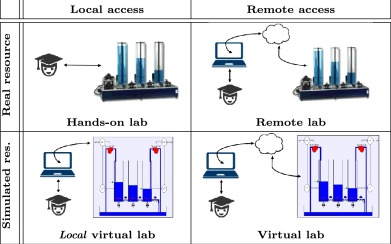
\includegraphics[width=0.65\textwidth]{figures/caracteristica_laboratories.jpg}
    \caption{Tipos de laboratórios consoante a localização, Heradio \textit{et al.} (2016), \cite{HERADIO20161}}
    \label{fig:classificaçãoHeratio}
\end{figure}

Representando de uma outra forma:
\begin{itemize}
    \item Acesso local
          \begin{itemize}
              \item Laboratório real: laboratório físico tradicional, onde os alunos podem realizar experiências práticas com equipamentos reais (amplamente utilizado em contexto de sala de aula de electrónica);
              \item Laboratório virtual local: um ambiente digital que simula um laboratório físico, permitindo aos alunos realizar experiências de forma virtual (durante a pandemia, os alunos utilizaram o \textit{multisim} instalado no computador para simular os circuitos);
          \end{itemize}
    \item Acesso remoto
          \begin{itemize}
              \item Laboratório remoto: um laboratório físico real que pode ser controlado à distância, permitindo aos alunos realizar experiências práticas sem estarem fisicamente presentes (nunca utilizado em contexto de sala de aula de electrónica);
              \item Laboratório virtual: um ambiente digital que simula um laboratório físico, permitindo aos alunos realizar experiências de forma virtual, independentemente da sua localização (utilizado, também, durante a pandemia mas na versão \textit{online} do \textit{multisim}).
          \end{itemize}
\end{itemize}

Também Zutin \textit{et al.} (2010) \cite{zutinlab2go}, citados por Zapata-Rivera e Larrondo (2017)~\cite{Zapata-Rivera}, classificam os laboratórios de forma idêntica, tal como representado na Figura~\ref{fig:classificaçãozutin}.

\begin{figure}[hbtp]
    \centering
    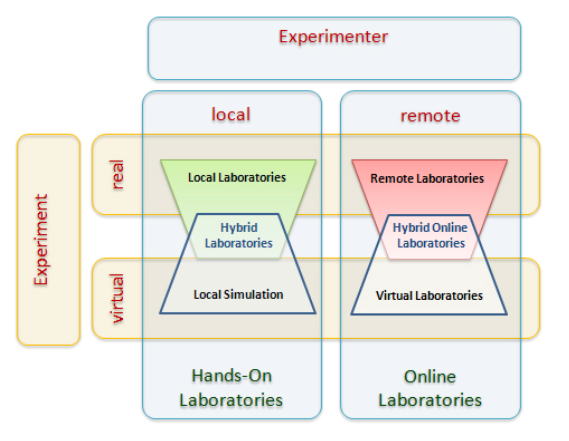
\includegraphics[width=0.65\textwidth]{figures/carac_lab.png}
    \caption{Tipos de laboratórios consoante a localização, segundo Zutin, \textit{et al.} \cite{zutinlab2go}}
    \label{fig:classificaçãozutin}
\end{figure}

Estas duas representações, no entanto, têm algumas diferenças ao nível da nomenclatura, sendo que os autores da segunda representação, introduzem os conceitos de \textit{Hybrid Laboratories} e \textit{Hybrid Online Laboratories}, tradução livre para laboratórios híbridos e laboratórios híbridos \textit{online}, respectivamente. Este tipo de laboratórios são criados através da combinação de laboratórios físicos e/ou laboratórios \textit{online}/remotos \cite{Zapata-Rivera}. Mais uma vez, não é propósito desta dissertação um estudo aprofundado destes conceitos. No entanto, apresentam-se dois casos de configurações híbridas, utilizadas com mais frequência em contexto de sala de aula:

\begin{itemize}
    \item Acesso a um laboratório real (no local) com acesso a um simulador local virtual (configuração realizada com bastante frequência em contexto de sala de aula, onde os alunos testam os circuitos no \textit{multisim} instalado no computador, antes de o testarem na placa branca);
    \item Acesso a um laboratório real (no local) com acesso a um laboratório virtual remoto (configuração usada e idêntica à anterior, com a diferença que o acesso ao laboratório virtual é feito através do \textit{multisim onnlie}.
\end{itemize}

O caso das configurações híbridas \textit{online} nunca foram utilizadas, uma vez que envolvem o acesso a laboratórios remotos e, como já foi referido, nunca foram utilizados  em contexto de sala de aula de electrónica.

\subsubsection{Uma questão de conceitos}
\label{sec:questaodeconceitos}
Como foi referido na nota\footref{Hofstein}, o estudo de Hofstein incide sobre os laboratórios de ciências. Sendo certo que as suas conclusões podem ser adaptadas ao contexto dos laboratórios no ensino da Electrónica, importa, daqui em diante, clarificar e distinguir os conceitos de ``laboratório virtual'' e ``simulador'' (válidos tanto para versões \textit{online} como locais), uma vez que estas duas definições tendem a sobrepor-se na maioria dos casos. Parte da literatura, trabalhos de investigação e fontes \textit{online} utilizam já o termo ``laboratório virtual'' \cite{BRINSON2015218, virtuallabng, EMaster2024May}, dado que a montagem nesses sistemas é concebida de forma a reproduzir, visual e funcionalmente, um ambiente laboratorial real. No entanto, o objectivo subjacente mantém-se: simular o comportamento de sistemas físicos ou electrónicos. Se se tomar como referência a representação da Figura~\ref{fig:classificaçãoHeratio}, apresentada por Heradio et al. (2016) \cite{HERADIO20161}, os laboratórios virtuais — quer sejam locais, quer \textit{online} — são considerados simuladores, uma vez que permitem simular o comportamento de sistemas físicos ou electrónicos, baseados em modelos matemáticos. No entanto, o inverso nem sempre é válido.

Apresentam-se de seguida três exemplos de tipos de laboratórios virtuais e simuladores (frequentemente utilizados em contexto de sala de aula), que ilustram a distinção entre o que se considera laboratório virtual e simulador, de acordo com a definição anteriormente enunciada. O Tinkercad \cite{tinkercad}, representado na Figura~\ref{fig:tinkercadVL}, é um simulador com características de laboratório virtual, uma vez que a representação dos componentes e a disposição do circuito se aproximam da realidade física de um laboratório tradicional. Por sua vez, o \textit{Multisim} \cite{multisim}, tanto na sua versão \textit{online} como na aplicação instalada no computador, representado na Figura~\ref{fig:multisimSimulador}, é um simulador, dado que a montagem dos circuitos é puramente esquemática, sem qualquer preocupação em replicar a aparência ou o contexto físico de uma bancada real.

\begin{figure}[hbtp]
    \centering
    \begin{subfigure}[hbtp]{0.48\textwidth}
        \centering
        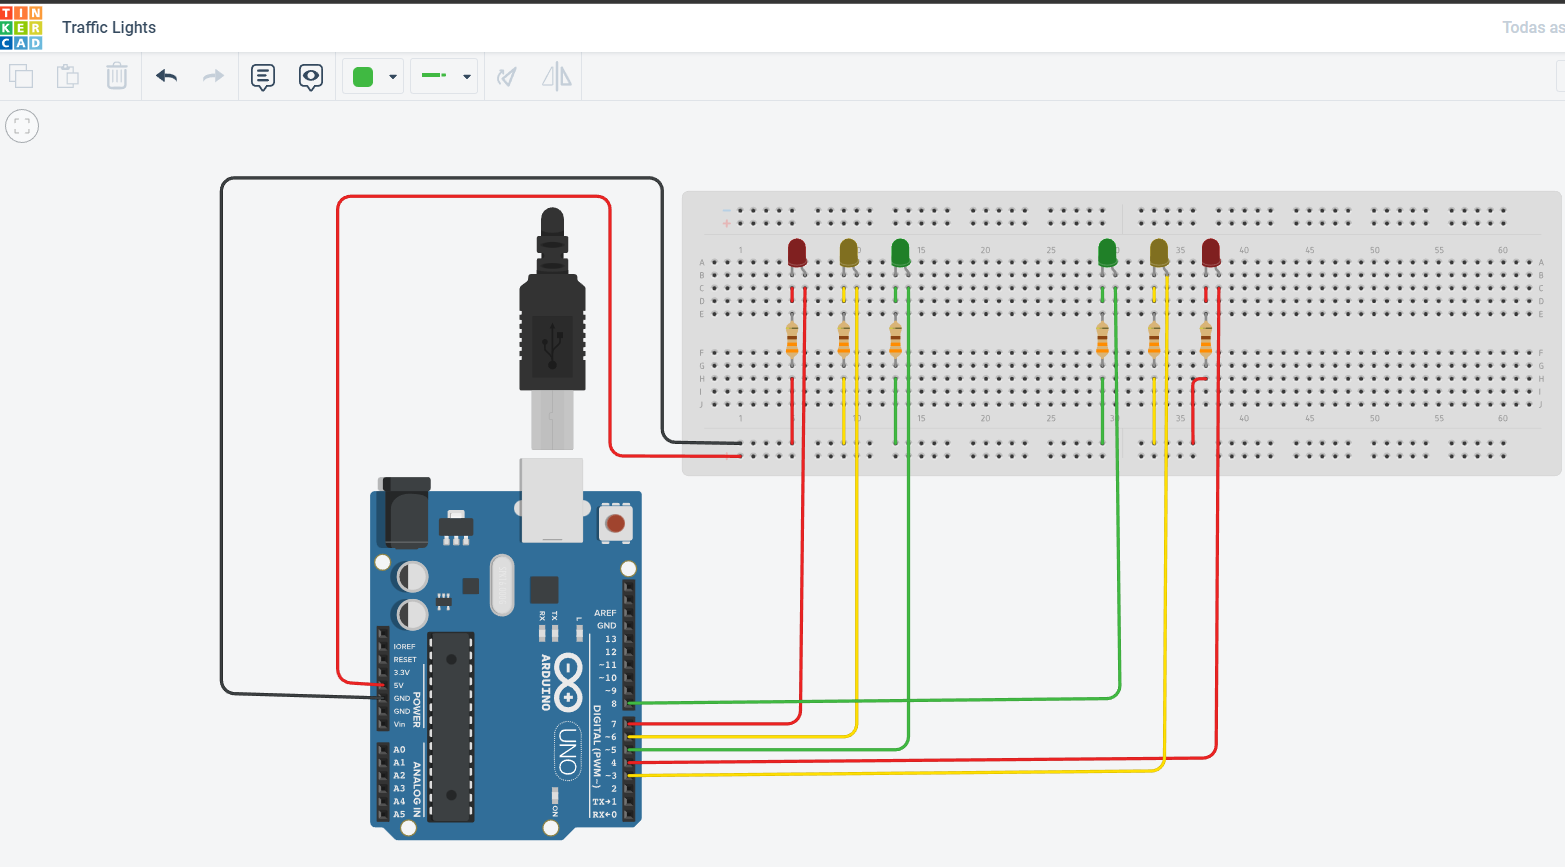
\includegraphics[width=0.9\textwidth]{figures/tinkercad_exemplo.png}
        \caption{\textit{Tinkercad} como laboratório virtual \cite{tinkercad}}
        \label{fig:tinkercadVL}
    \end{subfigure}
    \begin{subfigure}[hbtp]{0.48\textwidth}
        \includegraphics[width=0.9\textwidth]{figures/Astável-schematic.png}
        \caption{\textit{Multisim} como simulador \cite{multisim}}
        \label{fig:multisimSimulador}
    \end{subfigure}
    \caption{Laboratório virtual \textit{vs} simulador}
    \label{fig:tinkercad}
\end{figure}

O \textit{Falstad} \cite{falstad}, representado como exemplo na Figura~\ref{fig:falstad}, é outro dos simuladores \textit{online} amplamente utilizados em contexto des sala de aula. Ao contrário do \textit{Multisim}, que permite ao utilizador construir circuitos a partir de componentes e esquemas eléctricos, o \textit{Falstad} simula o comportamento de circuitos electrónicos com base em esquemas previamente desenhados e estruturados, frequentemente recorrendo a uma \textit{interface} mais simplificada e visualmente acessível. Este simulador é particularmente útil para introduzir conceitos fundamentais de Electrónica e teoria de circuitos, permitindo a visualização dinâmica de tensões, correntes e cargas, o que o torna uma ferramenta valiosa no ensino da electrónica.

\begin{figure}[hbtp]
    \centering
    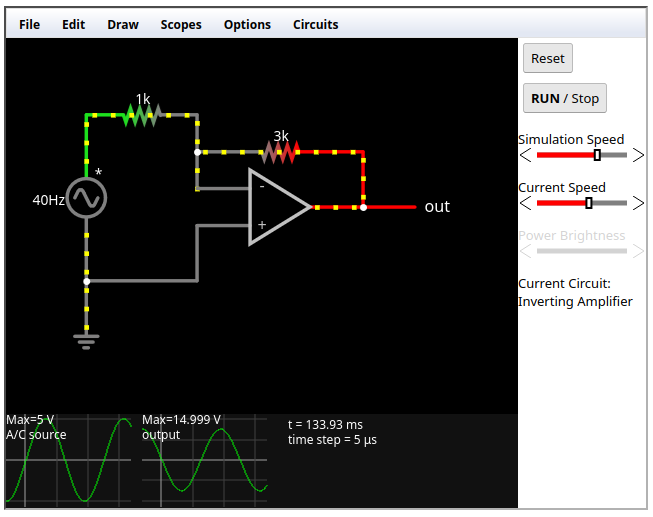
\includegraphics[width=0.6\textwidth]{figures/falstad.png}
    \caption{Simulador \textit{Falstad} (Exemplo) \cite{falstad}}
    \label{fig:falstad}
\end{figure}

Tal como foi referido anteriormente, não há um consenso na forma como são denominadas estas ferramentas. Faiña, (2022), \cite{faina}, refere-se ao \textit{Tinkercad} como sendo um simulador, ``Existem vários simuladores destinados a estudantes de eletrónica, como o \textit{TinkerCAD}''. No mesmo trabalho de investigação e refereindo-se ao \textit{Frizing}~\cite{fritzingdown}: ``O simulador apresentado neste artigo é implementado no \textit{Fritzing}(\ldots).''~\cite{faina}. Já Knörig, Wettach e Cohen, (2009), no seu artigo ''\textit{Fritzing: a tool for advancing electronic prototyping for designers}`` referem que ``(\ldots) decidiu permitir ao utilizador documentar o seu protótipo de trabalho baseado numa placa de ensaio com uma metáfora visual que imita a situação do utilizador no mundo real.''~\cite{Knorig2009Feb}. Além disso, ``(\ldots) um laboratório virtual pode ser definido como um ambiente no qual as experiências são conduzidas ou controladas parcial ou totalmente através de operação, simulação e/ou animação por computador, quer localmente, quer remotamente através da Internet.''~\cite{EvaluatingLearningExperiencesVirtualLaboratoryHongKong}. Os laboratórios virtuais oferecem aos alunos um conjunto de oportunidades diferentes, não só como substituto, mas também como complemento dos laboratórios reais.

Assim sendo, e sem prejuízo para os assuntos abordados nesta dissertação, é seguro afirmar que, na ausência de uma uniformização dos critérios relativos às definições e conceitos, todos os laboratórios virtuais podem ser considerados simuladores — reforçando, mais uma vez, que o contrário nem sempre é válido. Apesar disso, autores como Heying, Kejie e Jiang (2010) \cite{multisimVLHeying}, bem como Umenne e Hlalele (2020) \cite{multisimVLUmenne}, classificam o Multisim \cite{multisim} como um laboratório virtual nos respectivos trabalhos de investigação.

No contexto da Electrónica, e para efeitos desta dissertação, optar-se-á por distinguir os laboratórios virtuais como ambientes que procuram replicar visualmente os componentes e a disposição dos circuitos de acordo com a realidade física, ao passo que os simuladores serão entendidos como ferramentas cuja representação é puramente esquemática.

Após clarificada a distinção entre laboratórios virtuais e simuladores, importa agora enquadrar estes conceitos numa perspectiva particular, considerando os diferentes tipos de laboratórios já utilizados no ensino da electrónica. Cada uma destas tipologias possui características próprias, vantagens específicas e contextos de aplicação distintos, sendo particularmente relevantes no contexto do ensino da Electrónica e da abordagem \acrshort{stem}.

\subsubsection{Laboratório real}
%\textbf{link para não esquecer}
%https://digital.dge.mec.pt/laboratorios-de-educacao-digital
Neste tipo de laboratórios, os alunos têm à sua disposição os recursos, o equipamento e os materiais físicos necessários para realizar experiências, analisar dados, desenvolver competências de trabalho em equipa e cultivar o interesse pelas ciências. Estas competências revelam-se cruciais para muitas carreiras e profissões, especialmente nas áreas \acrshort{stem}. Além disso, os laboratórios podem ajudar a melhorar a compreensão dos alunos sobre o processo científico e a importância da investigação científica.

No caso específico do ensino secundário — e por experiência própria — uma das soluções encontradas para equipar e desenvolver os laboratórios passa pela aquisição de \acrshort{microcontroladores}, como o \gls{arduino}, o \gls{ESP32} ou o \gls{RaspberryPI}. Estes dispositivos, em conjunto com uma vasta gama de sensores disponíveis no mercado, são amplamente utilizados em ambientes educacionais e de investigação, permitindo a prototipagem rápida, a experimentação prática e a aprendizagem activa em disciplinas como a Electrónica. A principal vantagem prende-se com a relação custo-eficácia: os microcontroladores e os seus componentes associados são relativamente acessíveis, o que os torna viáveis mesmo em instituições com orçamentos limitados. Acresce a existência de uma comunidade de suporte activa e extensa documentação, factores que facilitam significativamente a aprendizagem e a implementação de projectos por parte de estudantes e docentes. Com estes dispositivos, é possível desenvolver uma variedade quase ilimitada de experiências, desde simples medições de temperatura até projectos avançados de automação, controlo e robótica educativa.
Em Portugal, esta vertente prática e experimental tem sido amplamente incentivada através de eventos e competições de robótica, que promovem o espírito inovador e empreendedor dos alunos, ao mesmo tempo que reforçam aprendizagens em contexto de sala de aula e de laboratório \cite{roboparty, fnr, cansat}. Entre as mais relevantes, destacam-se:
\begin{itemize}
    \item \textit{RoboParty};
    \item Festival Nacional de Robotica;
    \item \textit{Cansat}.
\end{itemize}

A eficácia do \gls{arduino} como ferramenta pedagógica tem sido amplamente documentada. Yoder (2015) \cite{yoder}, desenvolveu uma alternativa ao laboratório tradicional recorrendo ao \gls{arduino}: ``(\dots) a plataforma Arduino estimulou o interesse e o envolvimento dos alunos desde o início. Vários alunos começaram a alargar os projectos para além dos requisitos na terceira semana de aulas.''.

Graven, \textit{et al} (2018), \cite{graven}, citados por Plaza, \textit{et al.} (2018), \cite{plaza} destacam que ``(\ldots) No domínio da educação, o \gls{arduino} é também muito utilizado. Os estudantes de engenharia electrotécnica podem aceder a um laboratório compacto para trabalhar quando e onde quiserem.''. O mesmo autor refere ainda que ``(\ldots) Tal como foi demonstrado por muitas experiências e trabalhos, a robótica combinada com \acrshort{stem} constitui uma forma atractiva de transformar conceitos aborrecidos num processo de aprendizagem divertido.''.

Também Marzoli \textit{et al.} (2021), \cite{Marzoli}, no estudo intitulado ``Arduino: From Physics to Robotics'', exploram vários pontos e questões, entre os quais se o \gls{arduino} pode melhorar a prática laboratorial no ensino secundário italiano e mudar as atitudes dos alunos em relação às disciplinas \acrshort{stem}. Os autores questionam ``Como melhorar as práticas laboratoriais no ensino secundário, tendo em conta os orçamentos e as instalações limitadas disponíveis?''. As conclusões a que estes autores chegaram ajuda a revelar a potencialidade do \gls{arduino} em contexto laboratorial: ``A interação profícua entre professores com diferentes formações foi fundamental para a concepção de novas soluções e a exploração de novas aplicações.(\ldots) Assim, o \gls{arduino} pode ser considerado como uma espécie de micro-laboratório (\ldots)'' \cite{Marzoli}.

As possibilidades oferecidas por estes dispositivos — nomeadamente o \gls{arduino} — em contexto de sala de aula e como parte integrante de um laboratório são vastas, permitindo a realização de uma grande diversidade de projectos inovadores. Esta flexibilidade torna-o uma ferramenta valiosa para a educação e para a investigação, ao facilitar a aprendizagem prática e o desenvolvimento de competências em Electrónica e programação.

\subsubsection{Laboratório virtual - Acesso local e/ou remoto}
Um laboratório virtual é uma poderosa ferramenta que utiliza modelos matemáticos para emular dispositivos reais. Actualmente, os programas de simulação por computador são um padrão de desenvolvimento de produtos aceite pela indústria e são amplamente utilizados no ensino \cite{HERADIO20161, POTKONJAK2016309}.

A principal diferença entre os dois tipos de acesso aos laboratórios virtuais reside na forma como o utilizador acede ao programa. O \textit{Tinkercad} \cite{tinkercad}, representado como exemplo na Figura~\ref{fig:tinkercad}, é um dos laboratórios virtuais mais frequentemente utilizados em contexto de sala de aula. No entanto, está disponível apenas em versão online. Já o \textit{Fritzing} \cite{fritzingdown}, representado na Figura~\ref{fig:fritzing}, embora com capacidades de simulação mais limitadas, centra-se na prototipagem e visualização de circuitos. Ao contrário do \textit{Tinkercad}, só pode ser utilizado localmente, uma vez que não dispõe de versão online.

\begin{figure}[hbtp]
    \centering
    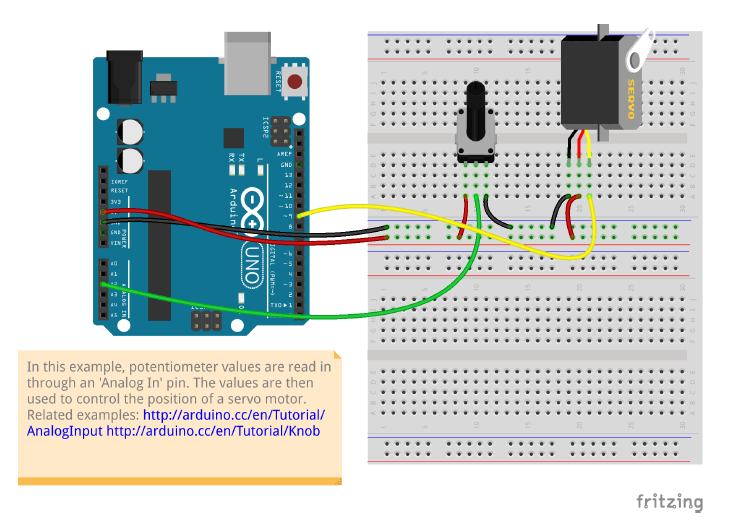
\includegraphics[width=0.6\linewidth]{figures/fritzing.png}
    \caption{Laboratório virtual \textit{Fritzing} exemplo}
    \label{fig:fritzing}
\end{figure}

Um laboratório virtual relativamente recente, apresentado como exemplo na Figura~\ref{fig:wokwi}, embora ainda pouco explorado, que pode constituir uma alternativa bastante interessante ao \textit{Tinkercad}, é o \textit{Wokwi} \cite{wokwi}. Este recurso permite simular diversas placas de desenvolvimento, como o \gls{arduino}, o \gls{ESP32}, o \textit{STM32}, o \gls{RaspberryPI}Pico, bem como uma vasta gama de sensores e actuadores \cite{wokwi}.

\begin{figure}[hbtp]
    \centering
    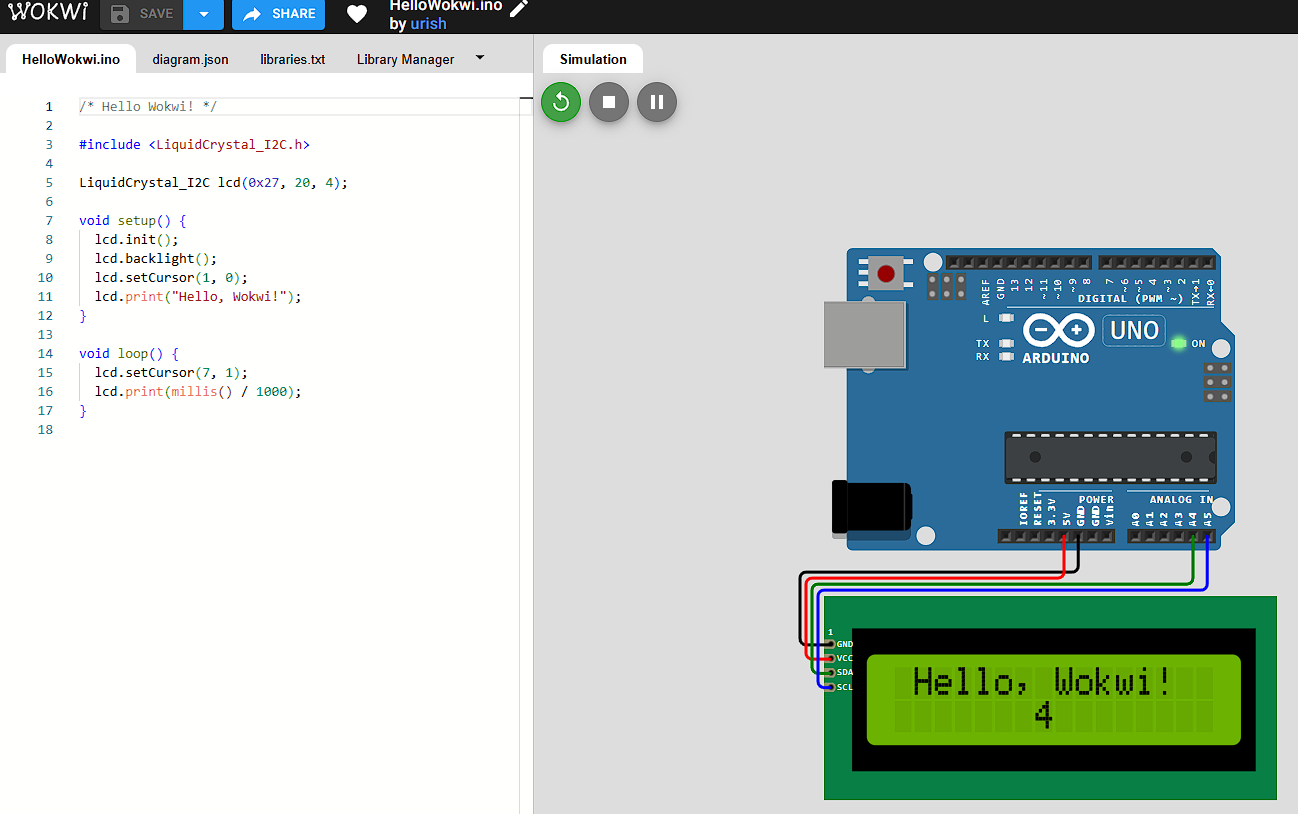
\includegraphics[width=0.6\linewidth]{figures/wokwi.png}
    \caption{Laboratório virtual \textit{Wokwi} exemplo}
    \label{fig:wokwi}
\end{figure}

Os laboratórios virtuais permitem a verificação e o ensaio de circuitos analógicos e digitais complexos. No caso do ensino secundário, por exemplo, plataformas como o \textit{Tinkercad} conseguem reproduzir componentes reais com um grau de precisão adequado a este nível de ensino. As faculdades e universidades de todo o mundo introduzem habitualmente este tipo de \textit{software} de simulação nos seus cursos de engenharia. Uma vez que todos os circuitos são virtuais, os estudantes podem trabalhar e experimentar uma vasta gama de elementos sem o risco de danificar ou destruir equipamento físico. Estes laboratórios virtuais oferecem, assim, um conjunto de oportunidades pedagógicas relevantes, não apenas como substituto, mas também como complemento aos laboratórios reais \cite{WebBrowserSimulators}. 

No caso concreto de uma turma com vinte ou mais alunos, por exemplo, torna-se mais seguro, numa primeira fase, simular circuitos que envolvam componentes como o \textit{TIP120}, o \textit{L293D} ou \acrshort{microcontroladores} como o \gls{arduino}, utilizando plataformas como o \textit{Tinkercad}. Esta abordagem permite aos alunos testar o funcionamento dos circuitos, identificar erros e compreender os princípios de controlo e potência em Electrónica básica, antes de avançarem para a montagem física dos projectos. Para além de preservar recursos e reduzir o risco de danos em equipamento real, esta estratégia promove uma aprendizagem mais segura, progressiva e eficaz. Mas as vantagens dos laboratórios virtuais vão muito para além das descritas anteriormente \cite{scheckler, lynch, BlogeMas95, vabtegensVL}. Estes laboratórios oferecem um ambiente seguro para a realização de experiências complexas e potencialmente perigosas, especialmente em fases introdutórias, reduzindo os riscos para estudantes e professores. Permitem ainda que os alunos progridam ao seu próprio ritmo e repitam as experiências tantas vezes quantas forem necessárias, uma vez que estão acessíveis em qualquer momento e a partir de qualquer lugar. Os laboratórios virtuais são, por natureza, mais económicos, de fácil instalação e manutenção. A estas vantagens acresce a vasta disponibilidade de informação, apoio técnico e tutoriais online que facilitam a sua integração no processo de ensino-aprendizagem.

No entanto, os laboratórios virtuais também apresentam algumas desvantagens. A principal prende-se com o desfasamento em relação à realidade. Retomando o exemplo anterior — a simulação de circuitos de potência —, o facto de não existirem consequências físicas reais pode induzir uma atitude de desresponsabilização ou falta de cuidado, levando o estudante a assumir que nada de grave poderá acontecer~\cite{POTKONJAK2016309}. Acrescem ainda os constrangimentos relacionados com a constante evolução tecnológica dos sistemas que suportam o laboratório virtual, bem como a necessidade de uma ligação à Internet estável e de qualidade. Quando o laboratório virtual não é utilizado em contexto de sala de aula, tende a reduzir-se a interacção directa entre os alunos e entre estes e os professores, uma vez que a comunicação ocorre sobretudo em ambiente \textit{online}. Além disso, exige-se do aluno um maior grau de autonomia e iniciativa. Há ainda vantagens que, em certos contextos, se podem transformar em desvantagens. Por exemplo, o facto de o aluno poder testar e simular sucessivas vezes sem penalização pode, a longo prazo, reduzir a sua sensibilidade e rigor no manuseamento de componentes reais. Da mesma forma, a imensa quantidade de informação disponível online exige do aluno uma capacidade de selecção crítica e filtragem informada~\cite{POTKONJAK2016309, vabtegensVL, Gherasim, Ghergulescu2019Feb}.

No caso de versão ser remota, as vantagens são semelhantes às de trabalhar com qualquer programa na nuvem:
\begin{itemize}
    \item Não há necessidade de instalar \textit{software} adicional no computador (versão \textit{online});
    \item Desde que a velocidade da Internet seja estável, o simulador pode ser acedido em qualquer lugar;
    \item Os circuitos são guardados e armazenados na nuvem;
    \item É ideal para trabalhos colaborativos e partilha de recursos.
\end{itemize}

\colorbox{yellow}{esta frase pode ficar mais à frente em jeito de conclusão}
Já foi visto na secção \ref{sec: remotelaboratory} - \textbf{REVER A REFERÊNCIA} que os resultados não são prejudicados pela utilização dos \acrshort{laboratório remoto}s. \textbf{IMPORTANTE - REferências - há um trabalho para apresentar como referência}

\subsubsection{Simuladores - Acesso local e/ou remoto}
Já foi referido na Secção~\ref{sec:questaodeconceitos} que os simuladores são ferramentas que permitem simular o comportamento de sistemas físicos ou electrónicos, sem a necessidade de replicar visualmente os componentes e a disposição dos circuitos. 

Um dos principais simuladores disponíveis gratuitamente, embora com algumas limitações funcionais, e utilizado regularmente em contexto de sala de aula, é o \textit{Multisim Online} \cite{multisim}. Durante os períodos de confinamento, este simulador revelou-se um verdadeiro ``salva-vidas''. Existe também uma versão \textit{premium}, que disponibiliza uma gama mais alargada de recursos \textit{online}, bem como uma versão que pode ser instalada localmente no \acrshort{pc}. O funcionamento destas duas versões é, na prática, idêntico, sendo que as diferenças situam-se ao nível da \textit{interface} gráfica e, sobretudo, na quantidade de recursos disponível, sendo que na versão local é obviamente muito mais extensa e completa, embora mais desactualizada (Para fins didácticos e educativos a que se propõe, revela-se extremamente eficaz.), como se pode ver na Figura~\ref{fig:multisimlocal} e Figura~\ref{fig:multisimremoto}.

\begin{figure}[hbtp]
    \centering
    \begin{subfigure}[hbtp]{0.48\textwidth}
        \centering
        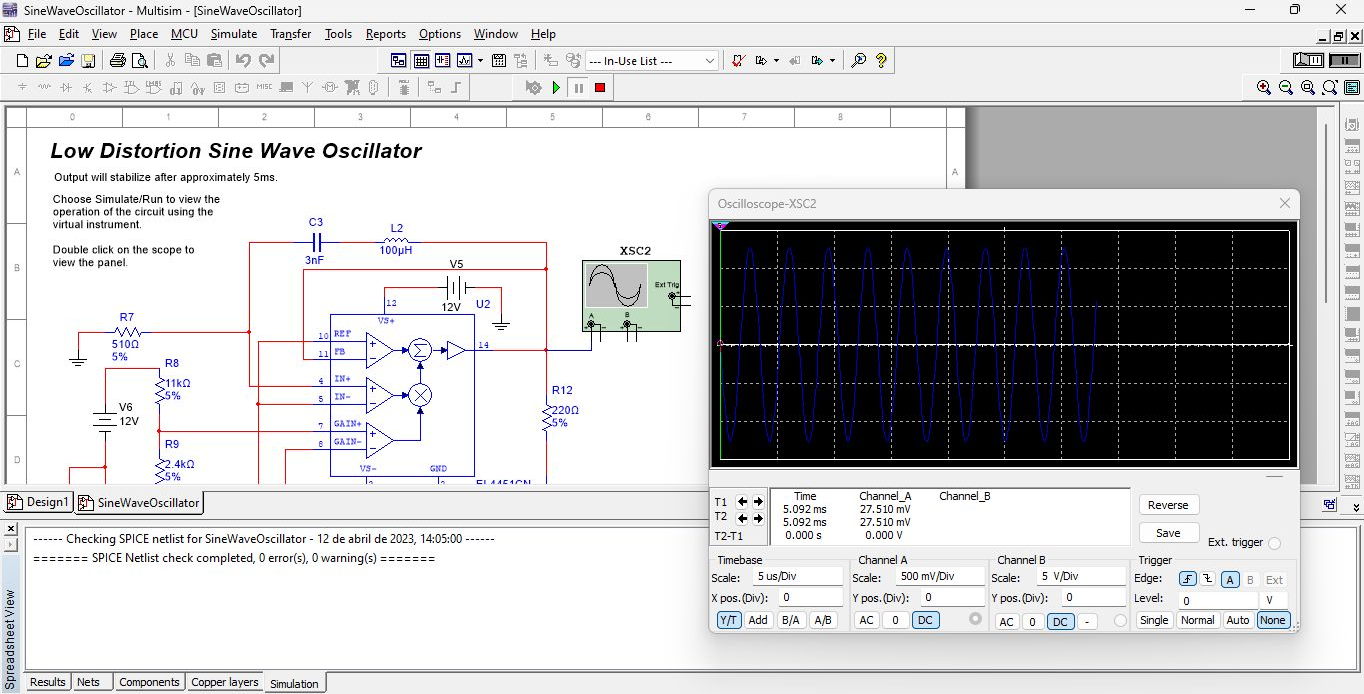
\includegraphics[width=0.9\textwidth]{figures/Multisim_Desktop.png}
        \caption{Local}
        \label{fig:multisimlocal}
    \end{subfigure}
    \begin{subfigure}[hbtp]{0.48\textwidth}
        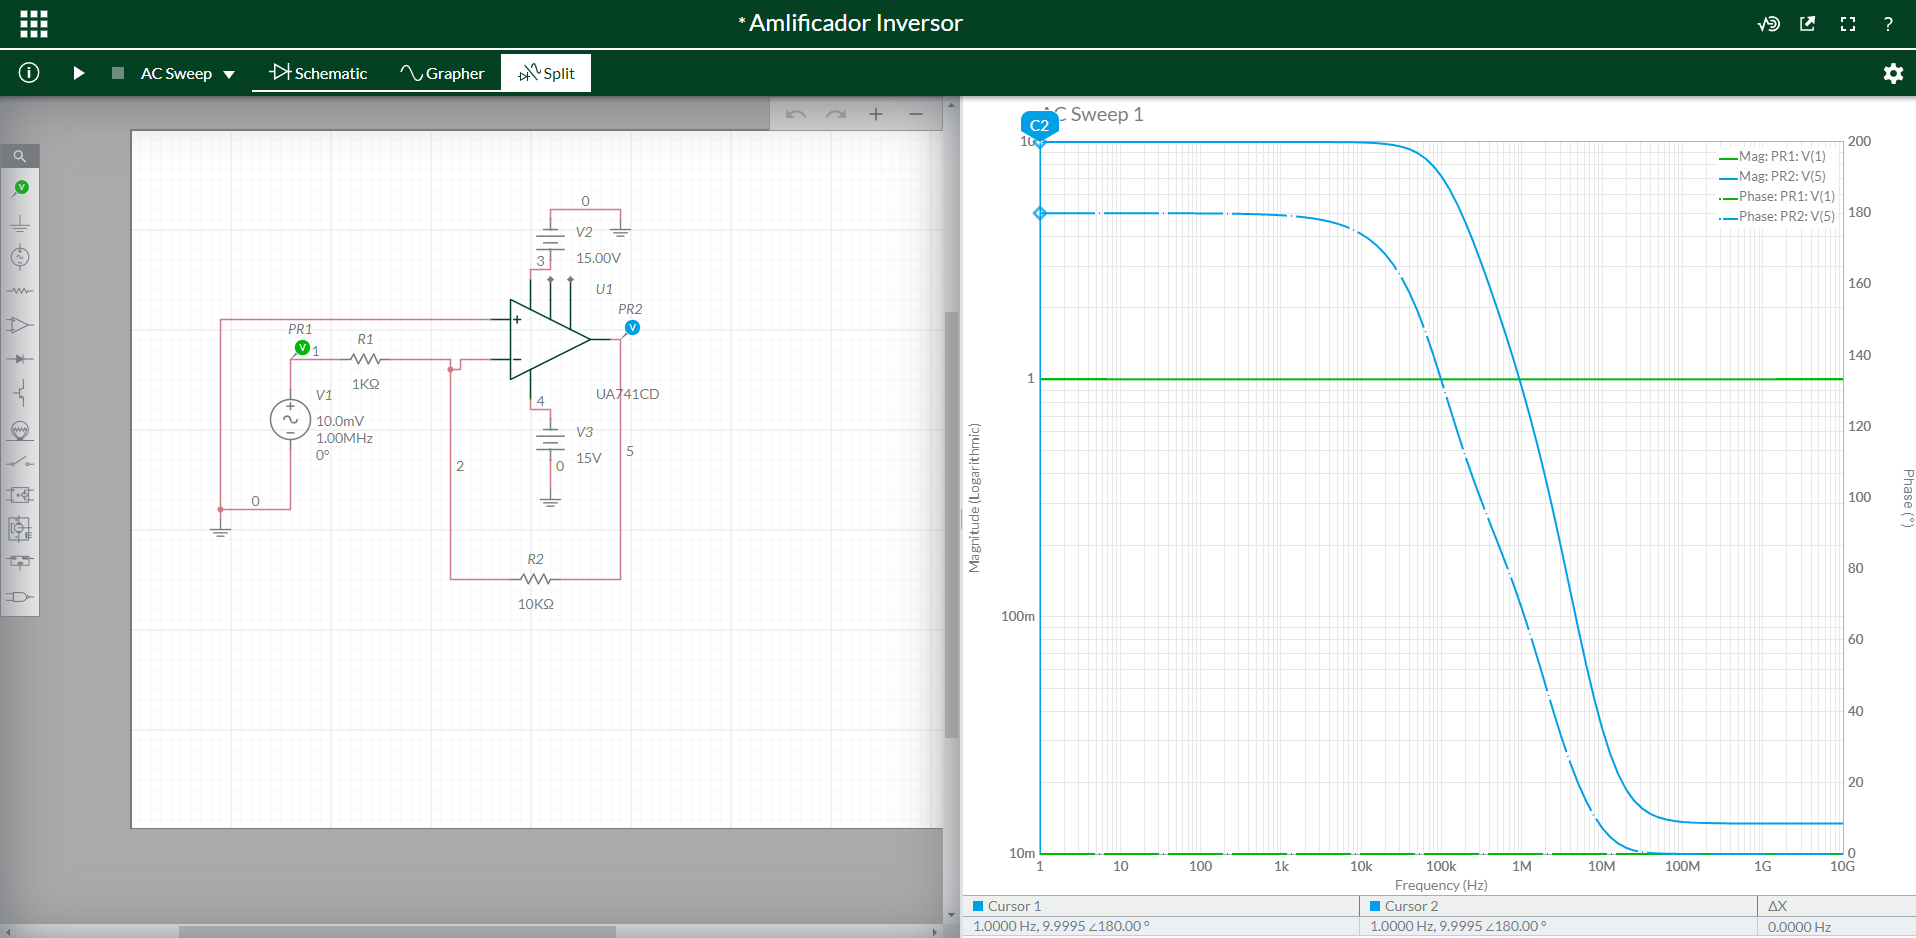
\includegraphics[width=0.9\textwidth]{figures/Multisim_ACsweep.png}
        \caption{Remoto}
        \label{fig:multisimremoto}
    \end{subfigure}
    \caption{Simulador \textit{Multisim}}
    \label{fig:multisimsimulator}
\end{figure}

Ainda assim, para os objectivos de estudo de circuitos simples, no âmbito do currículo do ensino secundário, qualquer das versões se revela adequada. Assim, sempre que for feita referência ao \textit{Multisim} \cite{multisim}, considerar-se-á, salvo indicação em contrário, que a afirmação se aplica a ambas as versões, sem prejuízo da generalidade.

Este \textit{software} integra a simulação virtual \acrfull{spice} padrão da indústria com um ambiente esquemático interativo para visualizar e analisar instantaneamente o comportamento de circuitos electrónicos. É uma ferramenta poderosa que utiliza modelos matemáticos para simular componentes reais, dispositivos ou circuitos com uma precisão muito boa, através de um navegador \textit{web}. Fornece uma plataforma para ``colmatar'' a lacuna entre a teoria dos manuais e os circuitos reais e também proporciona aos estudantes uma boa plataforma para experiências abrangentes e inovadoras \cite{multisim}. Além disso, dispondo de poderosas funcionalidades de aprendizagem e integração de \textit{hardware} de laboratório, o \textit{Multisim} ensina aos alunos conceitos fundamentais de eletrónica analógica, digital e de potência presentes em todo o currículo de engenharia e ciências~\cite{ImportantSimSoftware}.

Tomando novamente o exemplo de uma turma com vinte ou mais alunos, torna-se mais seguro simular circuitos de potência envolvendo componentes com \gls{triac}s, \gls{diac}s ou \gls{scr}s. Além disso, a possibilidade de simular circuitos complexos, como amplificadores operacionais, circuitos digitais e sistemas de controlo, torna o \textit{Multisim} uma ferramenta valiosa para a compreensão dos princípios fundamentais da Electrónica.

Citando Heying, Kejie e Li, (2010), ``(\ldots) podemos concluir que a criação de uma plataforma de simulação virtual através do \textit{Multisim} num computador permite construir facilmente todo o tipo de circuitos. (\ldots) Seguem-se os comentários de alguns alunos:''
\begin{itemize}
    \item ``O ensino experimental utilizando o \textit{Multisim} é uma boa abordagem para me ajudar a compreender as matérias;''
    \item ``Gostei de trabalhar na plataforma de simulação virtual \textit{Multisim}'';
    \item ``A simulação \textit{Multisim} ajudou-me a compreender melhor as experiências.''
\end{itemize}

Os mesmos autores concluem que: ``O laboratório virtual [\textit{Multisim}] desempenha um papel muito importante na atualização do método de ensino experimental, na melhoria da qualidade do ensino dos cursos em circuito e na otimização do efeito do ensino.'' \cite{heying}.

Outro simulador, representado como exemplo na Figura~\ref{fig:falstad}, e amplamente utilizado em contexto de sala de aula, foi criado e desenvolvido por \textit{Paul Falstad} em 1985, estando disponível em www.falstad.com \cite{falstad}. Trata-se de um simulador livre e de código aberto \cite{falstadlicenca}, que funciona directamente num navegador \textit{web} sob a forma de uma \textit{Java Applet}. A sua importância advém, em grande parte, da facilidade de interacção e da simplicidade com que representa circuitos eléctricos — aspectos particularmente relevantes na produção de recursos multimédia nas áreas da Electrónica e da Electricidade\footnote{Para maior rigor, importa referir que este recurso não se limita aos circuitos electrónicos, estando igualmente ligado a outras áreas da ciência, como a termodinâmica, a mecânica quântica, o processamento de sinal, entre outras \cite{falstadcompleto}.}. Além disso, o simulador \textit{Falstad} tem vindo a ser desenvolvido como uma aplicação de Internet há vários anos. De acordo com da Silva et al. (2011) \cite{RemoteTeachingElectricalCircuits}, citados por \textit{Falstad} (2024) \cite{falstad}, este simulador tem demonstrado versatilidade e aplicabilidade no ensino à distância.

O principal constrangimento prende-se com a ausência de parametrização avançada e de um modelo matemático robusto, o que faz com que este simulador não seja adequado para aplicações de engenharia profissional. No entanto, para fins didácticos e educativos, revela-se extremamente eficaz.

Por exemplo, como se pode observar na Figura~\ref{fig:falstad}, destacam-se as seguintes funcionalidades:

\begin{itemize}
    \item Os pontos amarelos animados representam a corrente eléctrica, cujo movimento demonstra o fluxo de cargas em ``tempo real'';
    \item A cor do fio varia entre verde e vermelho, consoante a direcção da corrente;
    \item Os componentes apresentam diferentes níveis de tensão;
    \item As formas de onda podem ser visualizadas directamente no circuito;
    \item É possível representar e controlar diferentes tipos de interruptores (por exemplo, para variar a frequência ou a tensão), o que permite ao utilizador observar fenómenos transitórios;
    \item A velocidade da simulação, bem como a intensidade da corrente, podem ser ajustadas.
\end{itemize}

Estas funcionalidades tornam o simulador Falstad uma ferramenta didáctica particularmente útil para introduzir conceitos fundamentais da Electrónica, como corrente, tensão, formas de onda e comportamento dinâmico de circuitos. A sua interface visual e interactiva contribui para uma melhor compreensão dos fenómenos eléctricos, mesmo por parte de alunos com conhecimentos ainda iniciais. Embora limitado em termos de precisão e análise avançada, o Falstad permite visualizar, de forma intuitiva e acessível, muitos dos princípios que são abordados nas aulas teóricas, servindo como uma excelente ponte entre a teoria e a prática, sobretudo em ambientes com recursos laboratoriais físicos reduzidos.

\colorbox{yellow}{\textbf{FALTA AQUI UMC CONCLUZÃOZINHA????????}}

\subsubsection{Laboratório remoto}
\label{sec: remotelaboratory}
Alguns dos constrangimentos associados aos laboratórios reais já foram abordados ao longo destes dois capítulos. As suas vantagens são evidentes, nomeadamente pela possibilidade de os alunos trabalharem com recursos físicos e concretos. No entanto, tanto no ensino secundário como no superior, nem sempre é viável garantir esse acesso. Por um lado, existem dificuldades associadas à obtenção de fundos para manter laboratórios devidamente equipados; por outro, é frequentemente incomportável montar um espaço que permita a realização de experiências em simultâneo por turmas com vinte ou mais alunos. No ensino superior, onde os estudantes são, pelo menos teoricamente, mais autónomos do que no ensino secundário, o principal obstáculo prende-se com a disponibilidade dos laboratórios fora do horário das aulas presenciais.

Numa época em que a tecnologia é cada vez mais encarada como um facilitador no processo de ensino/aprendizagem, a utilização de laboratórios remotos é cada vez mais comum e generalizada \cite{RemoteLabsImpactVISIR}. Além disso, os laboratórios remotos apresentam algumas vantagens em relação aos laboratórios reais e mesmo aos simuladores, tais como: flexibilidade, acessibilidade, disponibilidade e segurança~\cite{RemoteLabsImpactVISIR}.

Estes tipos de laboratórios - que incluem, por exemplo, o \acrshort{visir} ou o \textit{LabsLand}~\cite{labsland} - permitem que professores/investigadores e alunos acedam a equipamentos e/ou computadores através da Internet para realizar experiências e tarefas laboratoriais sem estarem no espaço físico dos laboratórios~\cite{ExperiencesRemoteLab}.

Num \acrshort{laboratório remoto}, a interação tem lugar à distância com a ajuda da infraestrutura remota. Esta é uma nova camada que se situa entre o utilizador e o equipamento do laboratório. É responsável pela transmissão das acções do utilizador e pela receção da informação sensorial do equipamento.
Várias investigações mostram que os estudantes podem efetivamente aprender com a utilização de laboratórios remotos e também de laboratórios virtuais, obviamente se estiverem empenhados no que estão a estudar \cite{RemoteLabsImpactVISIR}. Se se aplicar os conceitos abordados na Secção~\ref{sec:questaodeconceitos}, o \acrshort{visir} pode ser considerado um Laboratório remoto virtual, já que a \textit{interface} gráfica tenta replicar, visual e funcionalmente, um ambiente laboratoreal real, tal como representado na Figura~\ref{fig:exemplo_visir}. 

\begin{figure}[hbtp]
    \centering
    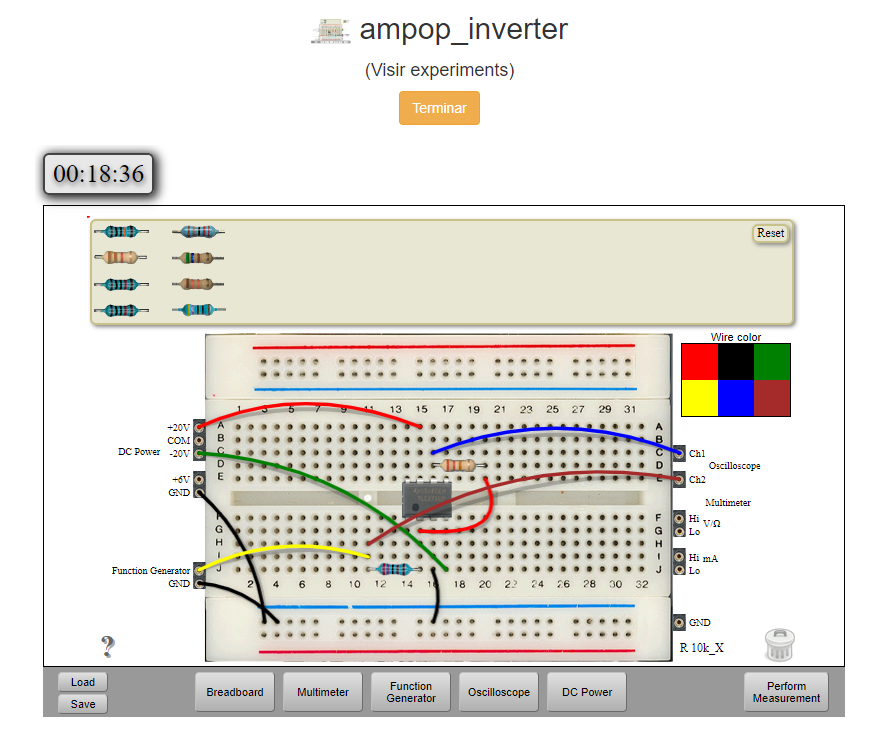
\includegraphics[width=0.4\linewidth]{figures/visir_sch.png}
    \caption{Exemplo \textit{\acrshort{visir}}}
    \label{fig:exemplo_visir}
\end{figure}

De acordo com Viegas \textit{et al.} (2018) \cite{ImpactRemoteLabTeachingPractices}, que citam Brinson (2015) \cite{BRINSON2015218} e Corter \textit{et al.} (2011) \cite{CORTER20112054}, os resultados obtidos com simuladores e laboratórios remotos podem ser considerados semelhantes - ou mesmo superiores - aos dos laboratórios práticos reais. No entanto, uma abordagem à aprendizagem laboratorial que utilize uma combinação de laboratórios práticos, simulações e procedimentos de laboratórios remotos parece ser a forma mais eficaz de aprendizagem, tirando partido dos benefícios dos três \cite{BRINSON2015218}.

Esta mesma conclusão foi obtida por de Mel e Samaranayaka (2017), no estudo intitulado ``\textit{Extending the boundaries of remote laboratory by providing hands on experience}''. Citando os autores: ``(\ldots) os estudantes estão disponíveis a usar o \acrshort{laboratório remoto} juntamente com o real (\ldots)'', mas ``(\ldots) não aconselham a total substituição (\ldots)''. O estudo conclui, ainda, que não há grande diferença entre o laboratório real e remoto, sendo que os conhecimentos adquiridos são (praticamente) os mesmos~\cite{deMel}.

Podem ser considerados outros estudos que, por exemplo, comparem laboratórios reais (práticos) e simulados, laboratórios reais e virtuais. De facto, Corter \textit{et al.} (2007) concluem que ``(\ldots) os laboratórios remotos e simulados podem ser pelo menos tão eficazes como os laboratórios práticos tradicionais no ensino de conceitos específicos da disciplina'' \cite{StudyRemoteHandsonSimulatedLabs}. Outro estudo feito por Kocijancic e O'Sullivan (2004) conclui que ``(\ldots) não se trata de saber se é melhor utilizar experiências reais ou laboratórios virtuais no ensino das ciências, uma vez que ambas as abordagens, utilizadas de forma complementar, podem contribuir para uma aprendizagem ativa mais eficaz.'' \cite{RealorVirtualDilema}. Tsihouridis \textit{et al.} (2019), concluem também que ``não há um vencedor final nesta controvérsia intemporal entre os dois ambientes de laboratório experimental, de acordo com a nossa investigação.'' \cite{controversy}.

VER O PARÁGRAFO SEGUINTE COM O PROF
Assim, através de estudos efectuados, será seguro afirmar que os laboratórios remotos são a melhor alternativa aos tradicionais em termos de baixo custo e ubiquidade, e algumas universidades já começaram a recorrer a laboratórios remotos nas suas sessões práticas \cite{VISIREngineeringPractices}. \textbf{\textcolor{red}{REVER esta frase em jeito de conclusão!}}

De facto, de acordo com Nafalski \textit{et al.}, (2010)\cite{ExperiencesRemoteLaboratories}, citando Auer e Gravier, (2009)\cite{ThemMnyfacesRemotLab} as razões para o crescimento dos laboratórios remotos em engenharia e ciência prendem-se com:

\begin{itemize}
    \item A crescente complexidade das tarefas de engenharia;
    \item O equipamento cada vez mais especializado e dispendioso, as ferramentas de software e os simuladores necessários;
    \item A necessidade de utilizar equipamentos e ferramentas de \textit{software}/simuladores dispendiosos em projectos com prazos curtos (como os apresentados em \cite{ExperiencesRemoteLab});
    \item A aplicação de equipamentos de alta tecnologia necessários em pequenas e médias empresas;
    \item A necessidade de pessoal altamente qualificado para controlar os novos equipamentos;
    \item As exigências da globalização e da divisão do trabalho.
\end{itemize}

No entanto, se se pretende, segundo Fan, Evangelista e Indumathi, (2021), \cite{EvaluationRemoteVirtualE-Learning}, citando Tawfik \textit{et al.}(2016)\cite{RemoteLabsImpactVISIR}, Chen \textit{et al.}, (2010)\cite{DevelopingVirtualAndRemoteUndergraduate} e Simão \textit{et al.}, (2014), \cite{RemoteLabsDevelopingCountries}, incorporar os laboratórios remotos com \gls{industria40}, já discutidas no Capítulo \ref{Capítulo1}, tem vantagens óbvias:
\begin{itemize}
    \item Os estudantes podem fazer os exercícios da disciplina ao seu próprio ritmo e de acordo com o seu nível de interesse;
    \item A quantidade de tempo (muitas vezes horas extraordinárias) que os professores têm de despender na preparação e ensino dos laboratórios pode ser reduzida;
    \item Podem ser efectuadas várias experiências utilizando a mesma configuração;
    \item Os laboratórios remotos permitem o acesso de um maior número de utilizadores, o que significa que a sua instalação acaba por ser mais barata do que a dos laboratórios físicos;
    \item Os laboratórios remotos estão acessíveis 24 horas por dia, 7 dias por semana;
    \item Os laboratórios remotos podem ajudar a reforçar o trabalho autónomo dos alunos;
    \item Os laboratórios remotos são mais seguros, tanto para o utilizador como para o equipamento ou software, uma vez que estão fisicamente separados e são orientados para a tecnologia.
\end{itemize}

Embora os laboratórios remotos ofereçam muitas vantagens, como as descritas em cima, é importante estar ciente das suas desvantagens (muitas delas comuns com as descritas para os laboratórios virtuais). A falta de interacção física directa, a dependência da ligação com a Internet, os desafios técnicos e de manutenção, a experiência de aprendizagem menos imersiva e a limitação da interação com colegas e professores são pontos críticos que devem ser considerados ao implementar esses laboratórios. No entanto, a principal desvantagem dos laboratórios remotos, prende-se com a complexidade da sua implementação. Como os \acrshort{laboratório remoto}s seguem uma arquitectura cliente-servidor, além do servidor é ainda necessário ter em conta a questão do \textit{hardware} e a sua integração com o \textit{software} que pode, ou não, ser proprietário. Há ainda a questão essencial da forma como os utilizadores acedem ao laboratório. Isto levanta problemas de largura de banda, que restringe o número de utilizadores que podem aceder simultaneamente ao \acrshort{laboratório remoto} \cite{HERADIO20161}.

Sendo assim, os laboratórios remotos não são simplesmente uma versão reduzida de um laboratório real (prático), mas uma abordagem diferente com pontos fortes e fracos alternativos, oferecendo novas oportunidades que não são proporcionadas pelas abordagens tradicionais. No final, se forem combinados e complementados com laboratórios reais e simulações, é possível tirar partido das vantagens que estes três tipos de laboratórios proporcionam.

%Quanto à implementação dum laboratório remoto, a quantidade de soluções que existem é vasta. 
Existem muitos tipos de laboratórios nos mais variados campos da ciência (Física, Electrónica, Robótica ou Química) e com os mais variados tipos de arquitectura de \textit{hardware} e \textit{software}. 

Dentro dos laboratórios remotos activos existentes e que abrangem as áreas \acrshort{stem}, destacam-se os seguintes:
\begin{itemize}
    \item \acrshort{visir} - é um \acrshort{laboratório remoto} que interliga vários componentes reais, que podem ser ligados para realizar diferentes tarefas e para construir circuitos específicos concebidos pelo utilizador final, como se pode ver na Figura \ref{fig:visirISEP}; permite a estudantes e professores fazerem medições reais em circuitos reais, algo que não é possível em simulações; será discutido com mais pormenor mais adiante;
    \item A Universidade de \textit{Deusto}, em Bilbao tem disponível uma conjunto de \acrshort{laboratório remoto}s, que inclui o \acrshort{visir}, o comando de um robô através de um \gls{arduino} ou a programação de uma \acrfull{fpga};
          %\textit{WebLab-Deusto} - O \textit{WebLab-Deusto} é uma iniciativa da Universidade de Deusto com o objetivo de aumentar a aprendizagem experimental através da utilização e desenvolvimento de laboratórios remotos
    \item \textit{iSES}\footnote{\url{https://www.ises.info/index.php/en/systemises/sdkisesstudio}} - tem várias experiências remotas que abrangem diversas áreas da ciências, como Física, Electrónica, Radioactividade, Electromagnetismo, etc.
    \item \textit{OpenSTEM}\footnote{\url{https://learn5.open.ac.uk/}} - estes laboratórios têm uma colecção de experiências abrangendo áreas científicas que vão desde a saúde, engenharia ou observatórios;
    \item \textit{Remote-LAB GymKT}\footnote{\url{http://remote-lab.fyzika.net/}} - Várias experiências que vão desde o controlo de um braço robótico através de um \gls{arduino} até experiências no campo da física e da electrónica;
\end{itemize}

\textbf{- Desenvolver um pouco mais o conceito de ``FEDERAÇÃO'' - PROF?? - retirei uma parte do texto. deixa de fazer sentido?}

\paragraph{VISIR}
\label{sec:visir}
No contexto desta dissertação, importa abordar o caso mais particular do \acrshort{visir}. De facto, este \acrshort{laboratório remoto} esteve na génese da criação do \acrshort{lare}. Além do mais, está disponível no \acrshort{isep}, Figura \ref{fig:visirISEP}. 

\begin{figure}[hbtp]
    \centering
    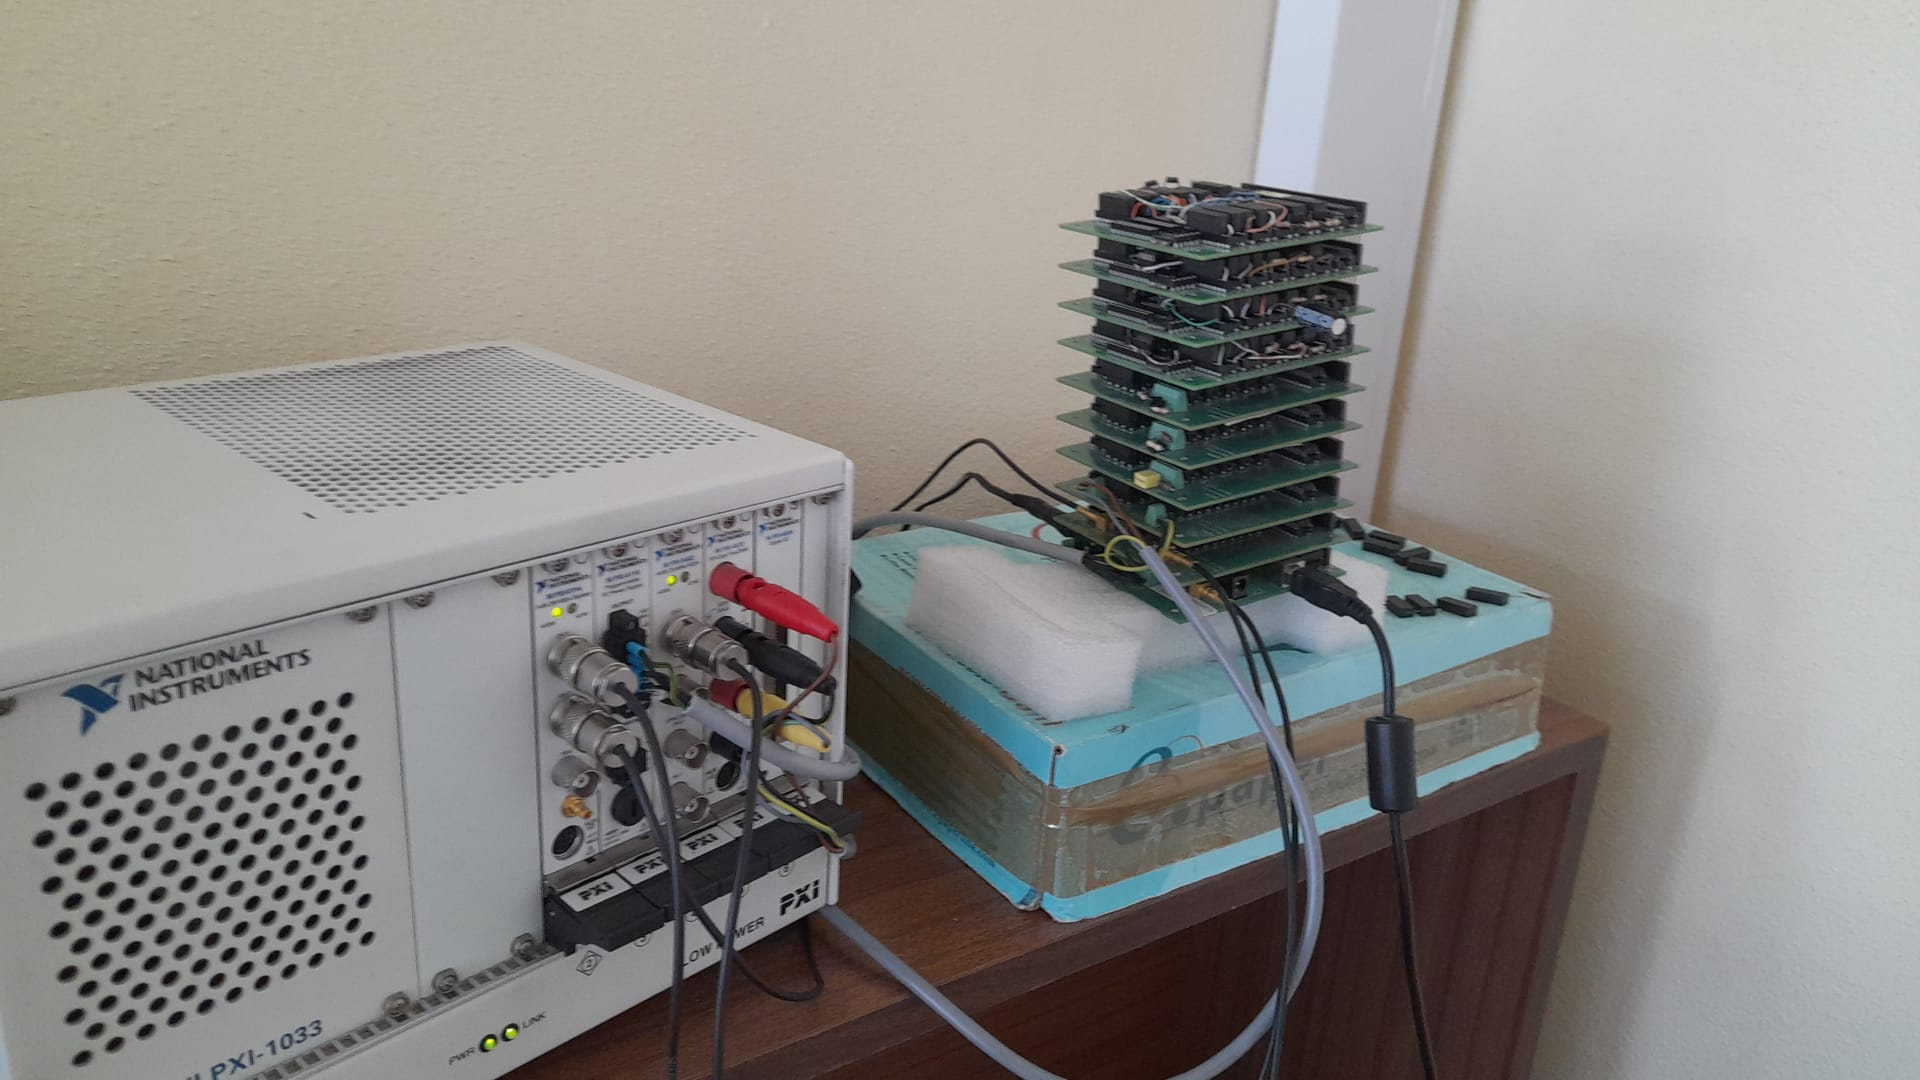
\includegraphics[width=0.75\textwidth]{figures/visirISEP.jpeg}
    \caption{\acrshort{visir} no \acrshort{isep}}
    \label{fig:visirISEP}
\end{figure}

O \acrshort{visir} é um \acrshort{laboratório remoto} para concepção, ligação e medição de circuitos electrónicos. O sistema \acrshort{visir} foi desenvolvido no \acrfull{bth}, \textit{Karlskrona}, Suécia, em 1999, e as suas funcionalidades e comunidade de utilizadores têm vindo a crescer desde então \cite{RemoteLabsImpactVISIR}. O projecto foi lançado no final de 2006 em conjunto com a \acrshort{ni}, nos \acrshort{eua}, (como fornecedor de instrumentos) e a \textit{Axiom EduTECH} na Suécia (como fornecedor de educação, \textit{software} técnico e serviços de engenharia para análise de ruído e vibrações). Foi apoiado financeiramente pela \acrshort{bth} e pela Agência Governamental Sueca para os Sistemas de Inovação (VINNOVA)\cite{VISIRExperiencesChallenges}.

Este sistema oferece aos estudantes a oportunidade de utilizarem recursos experimentais gratuitos 24 horas por dia, 7 dias por semana, sem um aumento significativo no custo por estudante. Com mais tempo dedicado a estas experiências, os estudantes tornam-se verdadeiros ''experimentadores``, capazes de criar bens e serviços que satisfaçam os requisitos de uma sociedade sustentável. Desta forma, o \acrshort{visir} não só melhora a aprendizagem, mas também contribui para a formação de profissionais comprometidos com o desenvolvimento sustentável \cite{OpenLabs77:online}.

Em 2018, tal como referido em \cite{PILARFederationVISIR}, o \acrshort{visir} já tinha sido implementado em 8 Instituições de Ensino Superior diferentes, situados em 6 países, incluindo o \acrshort{isep} (Portugal). No mesmo ano, segundo a mesma publicação, foram instalados novos sistemas em várias instituições da América do Sul. O software do \acrshort{visir} é lançado sob uma licença GNU GPL.

O conceito subjacente a este consiste em acrescentar uma opção de operação remota aos laboratórios de ensino tradicionais para os tornar mais acessíveis, independentemente dos alunos estarem no \textit{campus} ou principalmente fora do \textit{campus} \cite{TheVISIRproject}.

A arquitectura, do \acrshort{visir} pode ser dividida em quatro partes, tal como referido em \cite{tawfikexperiences} e como se pode ver na Figura~\ref{fig:platvisir} esta arquitectura inclui:
\begin{itemize}
    \item \textit{Equipment  Server} - Compreende todo o equipamento do \acrshort{visir} (módulos e \textit{chassis}): as placas \acrfull{pxi} e instrumentação (que estão ligadas à matriz de relés) controlados através do \acrshort{labview};
    \item \textit{Measurement Server} - Trata-se de um servidor escrito em Visual C++ para a \textit{Microsoft}. É programado por ficheiros ``max list'' que contêm os valores máximos dos componentes e ajustes dos instrumentos para cada experiência e servem para evitar a concepção de circuitos perigosos e proteger os instrumentos;
    \item \textit{Web Server} - Aloja a \textit{interface Web} do \acrshort{visir} e foi concebida em \textit{Apache} com uma base de dados em \textit{MySQL};
    \item \textit{Web Interface}, Figura \ref{fig:protoboadrvisir} - É o \textit{site} do \acrshort{visir} e foi escrito em PHP, com o cliente de experiências integrado escrito em \textit{Flash}.
\end{itemize}

\begin{figure}[hbtp]
    \centering
    \begin{subfigure}[hbtp]{0.48\textwidth}
        \centering
        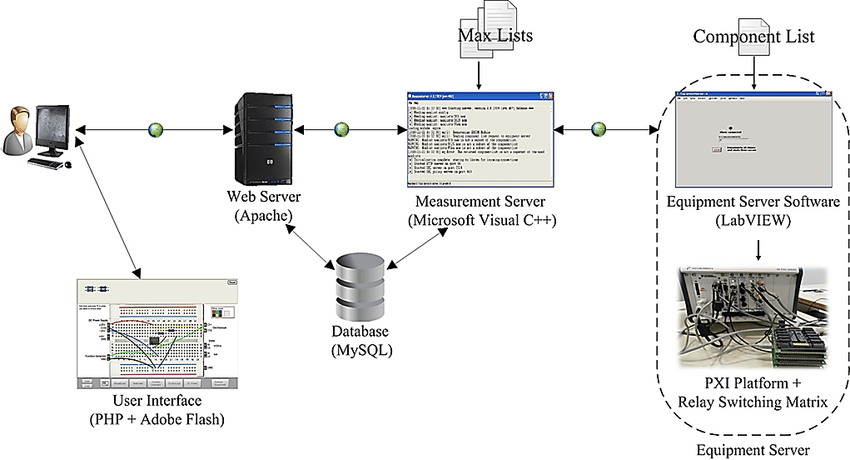
\includegraphics[width=0.9\textwidth]{figures/arquitectura_VISIR.png}
        \caption{Plataforma \acrshort{visir} \cite{tawfikexperiences}}
        \label{fig:platvisir}
    \end{subfigure}
    \begin{subfigure}[hbtp]{0.48\textwidth}
        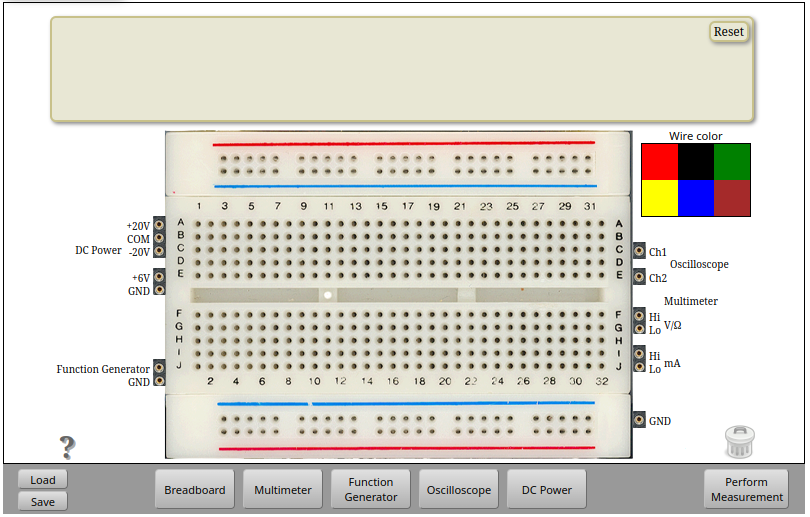
\includegraphics[width=0.9\textwidth]{figures/protboard_visir.png}
        \caption{\textit{Protoboard} \acrshort{visir}}
        \label{fig:protoboadrvisir}
    \end{subfigure}
    \caption{Arquitectura do \acrshort{visir}}
    \label{fig:arquitecturavisir}
\end{figure}

O \textit{chassis} PXI-1033 \cite{PXI-1033}, Figura~\ref{fig:PXI-1033}, é um controlador integrado com 5 \textit{slots} que foi concebida para aplicações de controlo remoto. Naturalmente, este dispositivo exige um \textit{interface} para \acrshort{pc}, que, neste caso, é feito através do \acrshort{labview}.

\begin{figure}[hbtp]
    \centering
    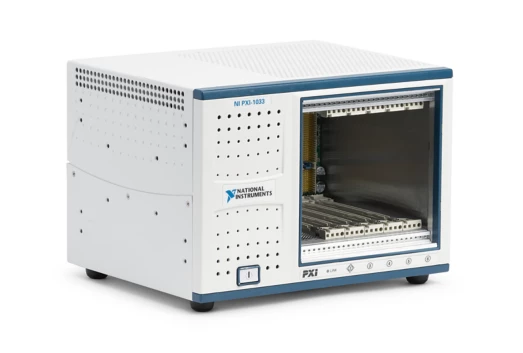
\includegraphics[width=0.4\textwidth]{figures/PXI-1033.png}
    \caption{\textit{Chassis} PXI-1033 \cite{PXI-1033}}
    \label{fig:PXI-1033}
\end{figure}

\textbf{NOTA: Neste momento estes chassis já não são fabricados e foram substituidos. Mantenho o texto como está ou devo colocar uma nota?}

Existem várias possibilidades de integração de módulos na PXI-1033, nomeadamente os que compõem o sistema \acrshort{visir}. Estes módulos podem variar consoante a configuração pretendida, estando disponíveis diversas opções adicionais no site oficial da National Instruments\footnote{\url{https://www.ni.com/en-us}}. No caso do \acrshort{visir}, os módulos utilizados são os seguintes:
\begin{itemize}
    \item Osciloscópio, PXI-5114, \SI{12}{\MHz}, 250 MS/s, 8-Bit, Figura \ref{fig:PXI-5114}
          \begin{figure}[hbtp]
              \centering
              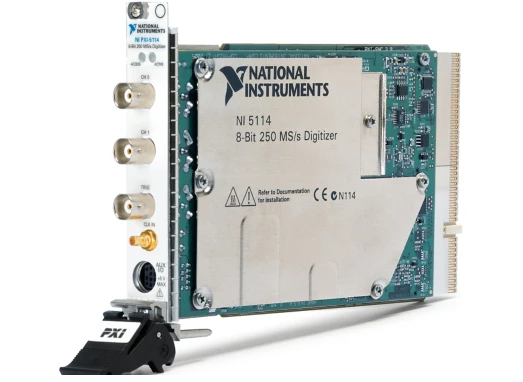
\includegraphics[width=0.4\textwidth]{figures/PXI-5114.png}
              \caption{Osciloscópio PXI-5114 \cite{PXI-5114}}
              \label{fig:PXI-5114}
          \end{figure}
    \item Gerador de sinal, PXI-5402, \SI{10}{\MHz} \textit{Bandwidth}, 1-\textit{Channel}, 14-Bit, Figura \ref{fig:PXI-5402}
          \begin{figure}[hbtp]
              \centering
              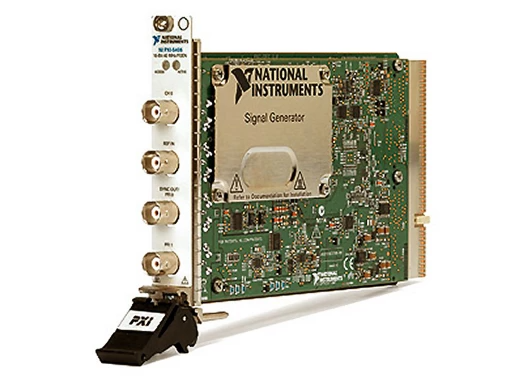
\includegraphics[width=0.4\textwidth]{figures/PXI-5402.png}
              \caption{Gerador de sinal PXI-5402 \cite{PXI-5402}}
              \label{fig:PXI-5402}
          \end{figure}
    \item Multímetro Digital, \(6^{1/2} \)Digitos, \(\pm\)\SI{300}{\volt}, \textit{Onboard} 1.8 MS/s Digitalizador isolado, suporte para medições de indutâncias e capacitâncias, Figura \ref{fig:PXI-4072};
          \begin{figure}[hbtp]
              \centering
              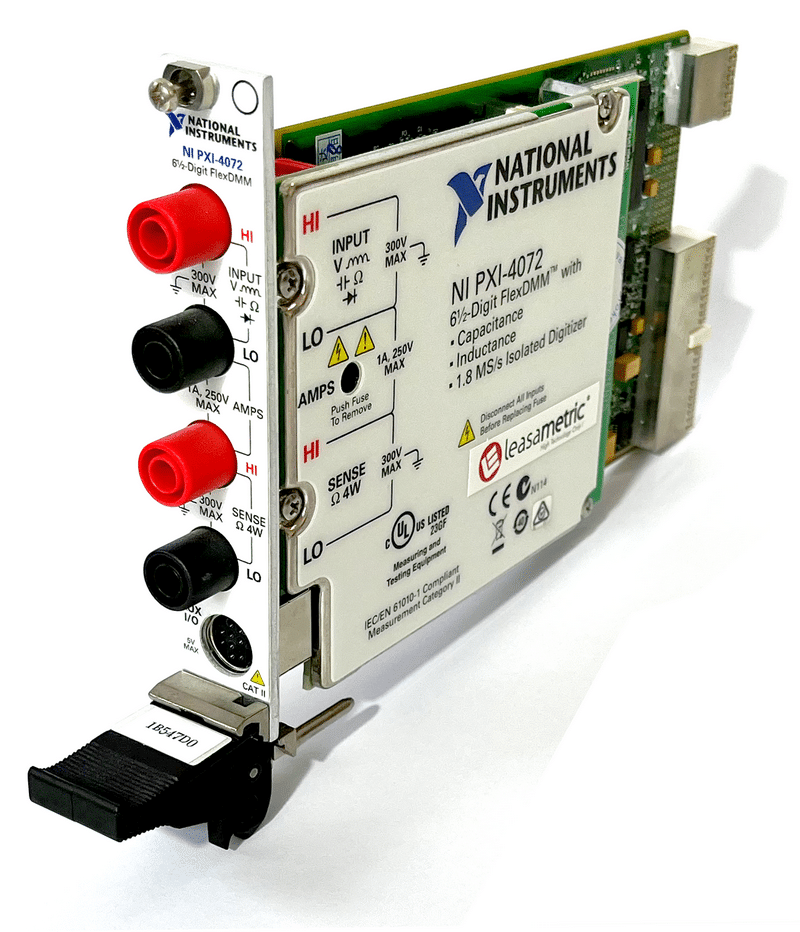
\includegraphics[width=0.3\textwidth]{figures/PXI-4072.png}
              \caption{Multímetro Digital PXI-4072 \cite{PXI-4072}}
              \label{fig:PXI-4072}
          \end{figure}
    \item Fonte de tensão programável, 3 canais, corrente de saída máxima de \SI{1}{\ampere}, gama de tensão de saída analógica: -\SI{20}{\volt} a \SI{20}{\volt}, Figura {\ref{fig:PXI-4110}}.
          \begin{figure}[hbtp]
              \centering
              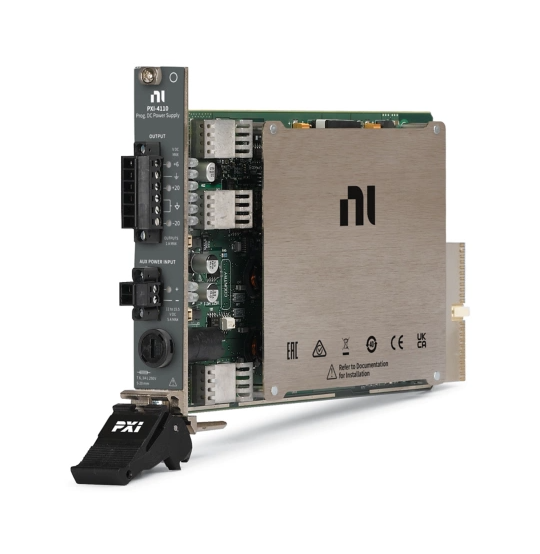
\includegraphics[width=0.4\textwidth]{figures/PXI-4110.png}
              \caption{Fonte de tensão PXI-4110 \cite{PXI-4110}}
              \label{fig:PXI-4110}
          \end{figure}
\end{itemize}

O \acrshort{visir} possuí uma \acrfull{mcr} concebida no \acrshort{bth} especialmente para o uso em experiências electrónicas em \acrshort{laboratório remoto}s tal como ser visto na Figura~\ref{fig:matrizvisir}. Esta matriz é constituída por quatro placas PC/104\footnote{\url{https://pc104.org/}} (de baixo para cima): fontes de tensão, multímetro digital, osciloscópio e a placa de topo permite configurar os componentes. A matriz é controlada por uma \acrfull{pic}, PIC18F4550 \cite{PIC18F4516datasheet}, montada na placa de alimentação (fontes de tensão) e comunica com um \acrshort{pc}, via \acrshort{usb}, e com os controladores das outras placas através das \acrshort{pic}s, PIC16F767 \cite{PIC16F7675datasheet}, via \acrfull{i2c}, montadas em cada placa \cite{matriz}.

\begin{figure}[hbtp]
    \centering
    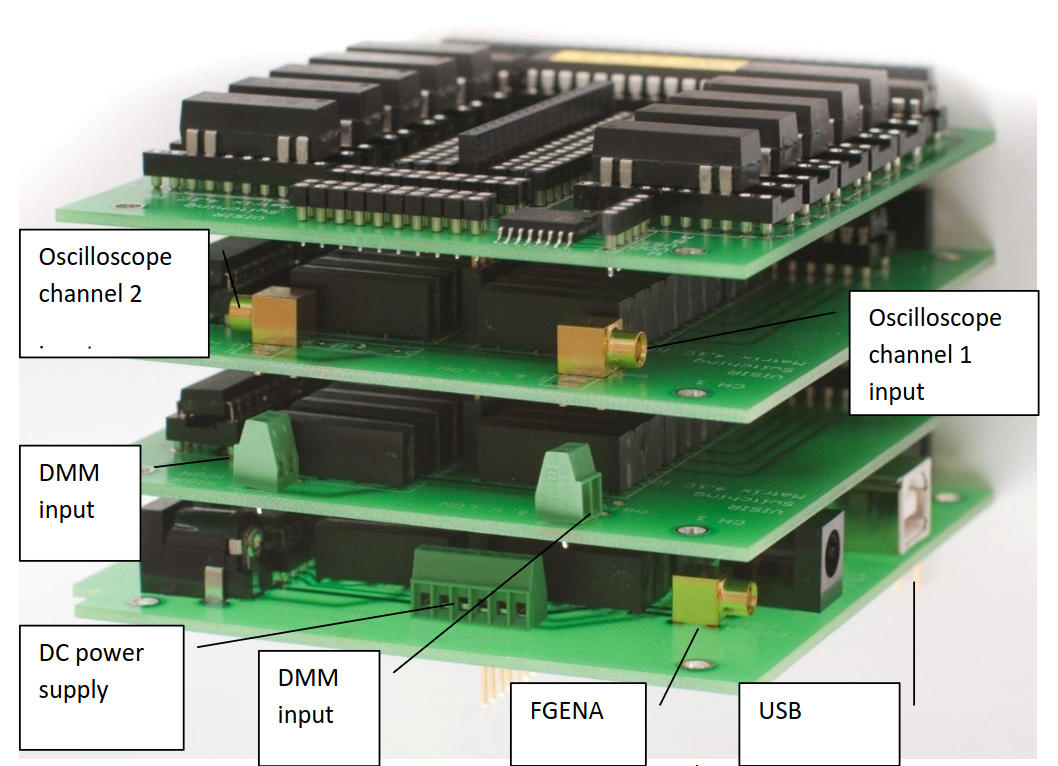
\includegraphics[width=0.4\textwidth]{figures/matriz.png}
    \caption{Matriz \acrshort{visir}\cite{matriz}}
    \label{fig:matrizvisir}
\end{figure}

Segundo Tawfik et al. (2012) \cite{tawfikexperiences} e Tawfik et al. (2013) \cite{tawfikvisir}, seis universidades já tinham implementado o \acrshort{visir}. No entanto, Pereira et al. (2017) referem que o \acrshort{visir} estava presente em 12 instituições e sete países \cite{pereira}.

Levanta-se, então, uma questão: Como fazer a integração de todos os \acrshort{laboratório remoto}s de forma a aproveitar os recursos e potenciar o trabalho colaborativo?

\paragraph{PILAR}
O projecto \textbf{\acrfull{pilar}} \textit{Erasums+}, foi iniciado em 2016 tendo terminado em 2019 e tinha como objectivo a criação de uma Federação de cinco nós \acrshort{visir} existentes, partilhando experiências, capacidade e recursos entre as diversas instituições e permitir o acesso ao \acrshort{laboratório remoto} \acrshort{visir}, através do consórcio \acrshort{pilar}, a estudantes de outras instituições de ensino \cite{garcia-loro}.

O \acrshort{visir} \acrfull{sig} é organizado para pessoas interessadas em Engenharia \textit{online} ou remota, especialmente na abertura de laboratórios universitários para acesso remoto 24/7. Este projeto foi lançado com o objetivo de divulgar métodos de abertura de laboratórios para acesso remoto,  partilhar ideias, equipamento e material didático, bem como de discutir o desenvolvimento da plataforma \acrshort{visir}. Outro dos objetivos é a padronização de bancos de trabalho \textit{online} localizados em universidades de todo o mundo, constituindo laboratórios de rede disponíveis para sessões de laboratório para estudantes dentro e fora do \textit{campus} \cite{visirsig}.

A missão da Federação \acrshort{visir} é actualizar e alargar o \acrshort{visir} \acrshort{sig}, integrando indivíduos e instituições. O objetivo é fornecer um sistema uniforme, em que os estudantes se possam registar e utilizar os laboratórios federados baseados no \acrshort{visir} e os materiais de aprendizagem de diferentes instituições pertencentes à Federação. Através de um mecanismo comum partilhado, deverá ser possível aceder a cada experiência a partir de um único sistema de gestão da aprendizagem. Os principais objectivos da Federação são \cite{visirfederation}:
\begin{itemize}
    \item Expandir o \acrshort{sig} a instituições;
    \item Conectar todos os nós \acrshort{visir};
    \item Alargar a gama de aplicações;
    \item Melhorar a utilização do \acrshort{visir};
    \item Promover o laboratório remoto \acrshort{visir};
    \item Partilhar materiais de aprendizagem;
    \item Trocar experiências entre os detentores e utilizadores do \acrshort{visir}.
\end{itemize}

Como se viu anteriormente, o \acrshort{visir} funciona numa base de cliente-servidor, o que significa que, se um determinado servidor não estiver disponível, também o laboratório não estará. Neste caso, a Federação permite o redireccionamento dos pedidos dos clientes para um outro nó \acrshort{visir} que esteja disponível \cite{kreiter}.
